\documentclass[a4paper, 11pt, oneside, polutonikogreek, german]{article}
\usepackage{gfsbaskerville}
% Load encoding definitions (after font package)
\usepackage[LGR,T1]{fontenc}
\usepackage{textalpha}

\usepackage{listings}
\lstset{basicstyle=\ttfamily}

% Babel package:
\usepackage{babel}
\usepackage{yfonts}
% With XeTeX$\$LuaTeX, load fontspec after babel to use Unicode
% fonts for Latin script and LGR for Greek:
\ifdefined\luatexversion \usepackage{fontspec}\fi
\ifdefined\XeTeXrevision \usepackage{fontspec}\fi

% "Lipsiakos" italic font `cbleipzig`:
\newcommand*{\lishape}{\fontencoding{LGR}\fontfamily{cmr}%
		       \fontshape{li}\selectfont}
\DeclareTextFontCommand{\textli}{\lishape}

\usepackage{booktabs}
\setlength{\emergencystretch}{15pt}
\usepackage{fancyhdr}
\usepackage{microtype}
\usepackage[titles]{tocloft}
\usepackage{sectsty}

\usepackage[dvipsnames]{xcolor}
\usepackage{eso-pic,graphicx}
\usepackage[top=40mm, bottom=35mm, outer=45mm, inner=45mm]{geometry}
\setlength{\columnsep}{90pt}

\definecolor{customColor}{RGB}{244, 245, 240}

\usepackage{setspace}
\onehalfspacing

\allsectionsfont{\swabfamily}
\sectionfont{\swabfamily\Huge}
\subsectionfont{\swabfamily\LARGE}
\subsubsectionfont{\swabfamily\LARGE}
\paragraphfont{\swabfamily\LARGE}
% change color of text, example replace all \color{Goldenrod} with \color{lightgray}

\makeatletter % change only the display of \thepage, but not \thepage itself:
\patchcmd{\ps@plain}{\thepage}{\color{customColor}{\thepage}}{}{}
\makeatother

\color{customColor}

\begin{document}
\swabfamily
\renewcommand{\contentsname}{
\swabfamily{Inhaltsverzeichnis}
}

\renewcommand{\cftsecfont}{\swabfamily}
\renewcommand{\cftsubsecfont}{\swabfamily}
\renewcommand{\cftsubsubsecfont}{\swabfamily}

% fix toc page numbers
\let\origcftsecfont\cft
\let\origcftsecpagefont\cftsecpagefont
\let\origcftsecafterpnum\cftsecafterpnum
\renewcommand{\cftsecpagefont}{\swabfamily{\origcftsecpagefont}}
\renewcommand{\cftsecafterpnum}{\swabfamily{\origcftsecafterpnum}}
\let\origcftsubsecpagefont\cftsubsecpagefont
\let\origcftsubsecafterpnum\cftsubsecafterpnum
\renewcommand{\cftsubsecpagefont}{\swabfamily{\origcftsubsecpagefont}}
\renewcommand{\cftsubsecafterpnum}{\swabfamily{\origcftsubsecafterpnum}}
\let\origcftsubsubsecpagefont\cftsubsubsecpagefont
\let\origcftsubsubsecafterpnum\cftsubsubsecafterpnum
\renewcommand{\cftsubsubsecpagefont}{\swabfamily{\origcftsubsubsecpagefont}}
\renewcommand{\cftsubsubsecafterpnum}{\swabfamily{\origcftsubsubsecafterpnum}}

\renewcommand\thefootnote{\swabfamily{\arabic{footnote}}}
\let\oldfootnote\footnote
    \renewcommand{\footnote}[1]{\oldfootnote{#1}}
\AddToShipoutPictureBG{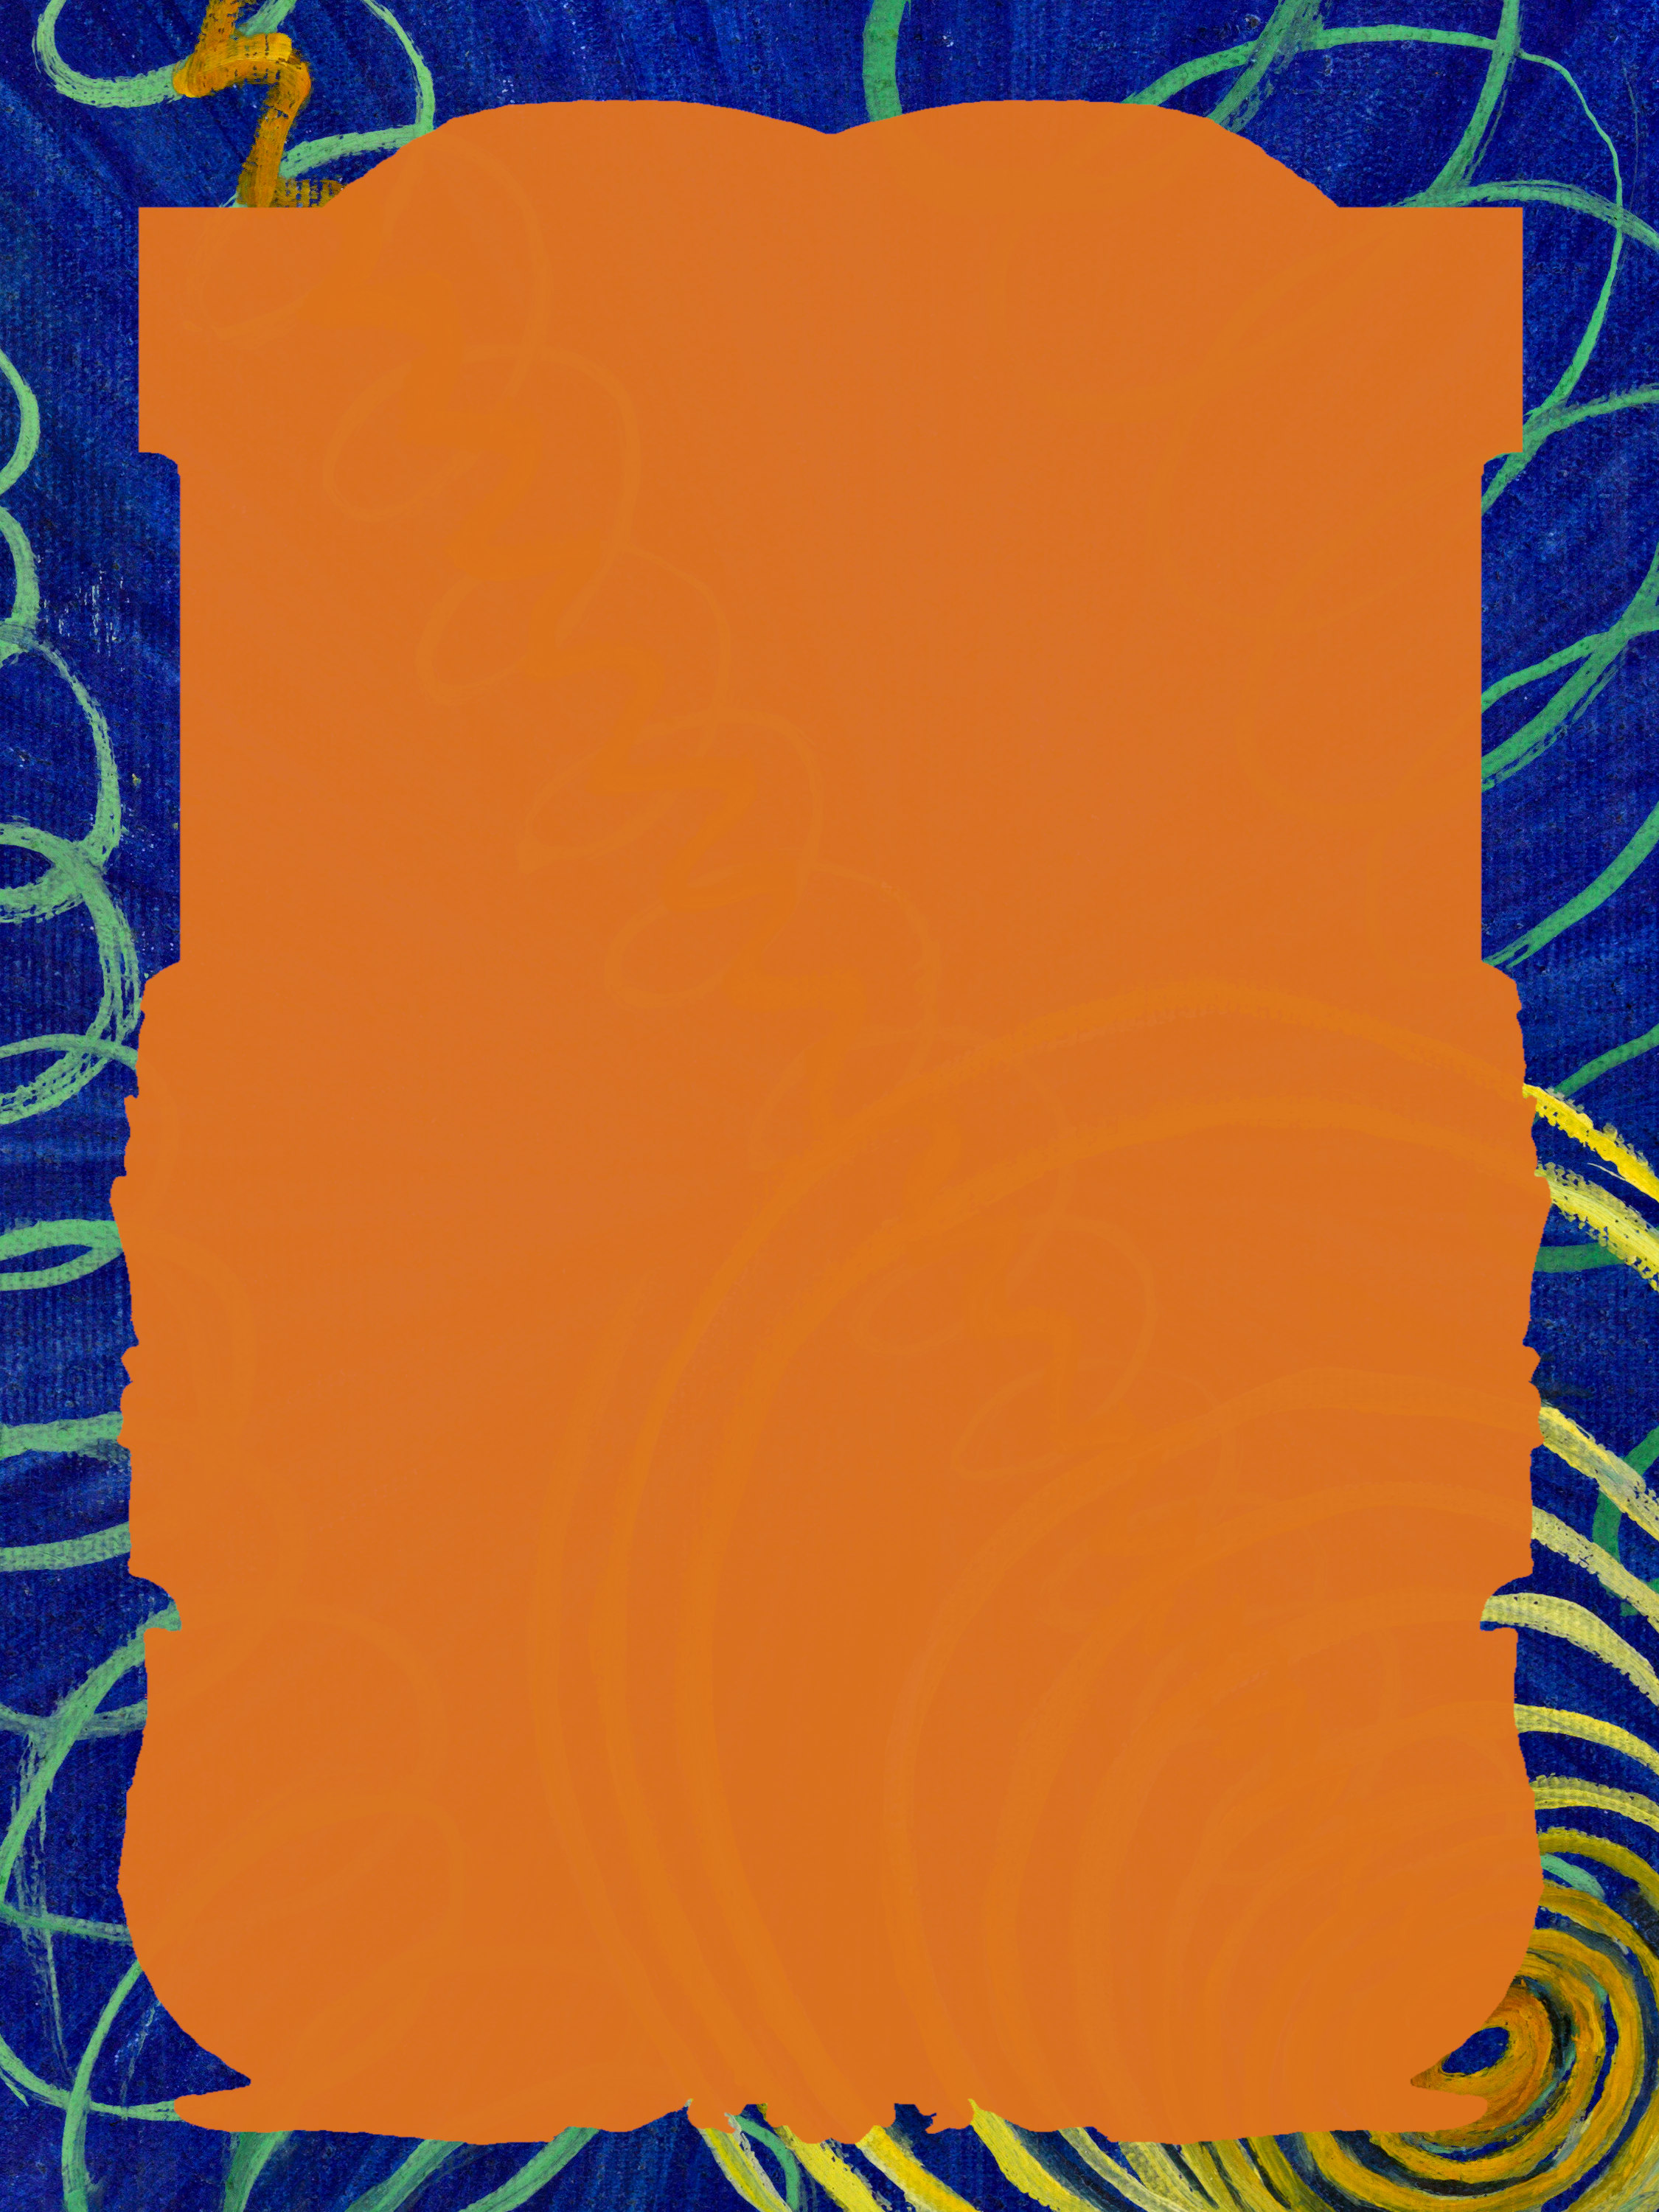
\includegraphics[width=\paperwidth,height=\paperheight]{klint2.jpeg}}
\begin{titlepage} % Suppresses headers and footers on the title page
	\centering % Centre everything on the title page
	%\scshape % Use small caps for all text on the title page

	%------------------------------------------------
	%	Title
	%------------------------------------------------
	
	\rule{\textwidth}{1.6pt}\vspace*{-\baselineskip}\vspace*{2pt} % Thick horizontal rule
	\rule{\textwidth}{0.4pt} % Thin horizontal rule
	
	\vspace{1\baselineskip} % Whitespace above the title
	
	{\scshape\Huge "Uber den Ursprung der von Pallas gefundenen und anderer ihr "ahnlicher Eisenmassen,\\ und "uber einige damit in Verbindung stehende Naturerscheinungen.}
	
	\vspace{1\baselineskip} % Whitespace above the title

	\rule{\textwidth}{0.4pt}\vspace*{-\baselineskip}\vspace{3.2pt} % Thin horizontal rule
	\rule{\textwidth}{1.6pt} % Thick horizontal rule
	
	\vspace{1\baselineskip} % Whitespace after the title block
	
	%------------------------------------------------
	%	Subtitle
	%------------------------------------------------
	
	{\scshape \Large Von Ernst Florens Friedrich Chladni,} % Subtitle or further description
	
	\vspace*{1\baselineskip} % Whitespace under the subtitle
	
        {\scshape in Wittenberg, der Phil. und Rechte Doktor, der Berliner Gesellschaft Naturf. Freunde Mitgliede, und der k"onigl. Societ"at der Wissenschaften zu G"ottingen Korrespondenten.} % Subtitle or further description
    
	%------------------------------------------------
	%	Editor(s)
	%------------------------------------------------
        \vspace*{\fill}

	\vspace{1\baselineskip}

	{\small\scshape Riga 1794.}
	
	{\small\scshape{Bei Johann Friedrich Hartknoch}}
	
	\vspace{0.5\baselineskip} % Whitespace after the title block

        \scshape Internet Archive Online Edition  % Publication year
	
	{\scshape\small Namensnennung Nicht-kommerziell Weitergabe unter gleichen Bedingungen 4.0 International} % Publisher
\end{titlepage}
\setlength{\parskip}{1mm plus1mm minus1mm}
\clearpage
\LARGE
\pagestyle{fancy}
\fancyhf{}
\cfoot{\swabfamily{\thepage}}
\tableofcontents
\clearpage
\section{Der gefundene Stoff niedergefallener Feuerkugeln, und die Pallasische wie auch andere ihr "ahnliche Massen sind ganz einerlei.}
\paragraph{}
Da die meisten bisherigen Behauptungen "uber den Ursprung der von Pallas in Sibirien gefundenen und einiger ihr "ahnlicher Eisenmassen mit den Eigenschaften und mit den Lokalumst"anden derselben gar nicht zusammentressen wollten: so dachte ich einer andern Erkl"arungsart nach, und kam endlich auf eine, welche sich mit deren Eigenschaften und Ortsumst"anden vollkommen vereinen l"asst, und zugleich "uber einige andere ebenfalls noch auf keine befriedigende Art erkl"arte Naturerscheinungen ein viel helleres Licht verbreitet. So sehr meine neue Erkl"arungsart manchem anfangs paradox scheinen m"ochte, so wenig wird sie es ihm dann noch sein, wenn er meine Gr"unde gegen die bisherigen und f"ur meine Behauptungen ohne vorgefasste Meinung erwogen haben wird. Allem Ansehen noch sind n"amlich diese Massen und der Stoff der Feuerkugeln ganz einerlei: Alles, was man an diesen vor und nach ihrem Niederfallen bemerkt hat, lehrt uns, dass sie aus schweren und dichten Grundstoffen bestehen, die weder als dichte Masse durch irgend eine tellurische Kraft in die H"ohe gef"uhrt, noch aus den in der Atmosph"are befindlichen Teilen angeh"auft sein konnten, sondern aus dem "ubrigen Weltraume zu uns anlangten, und l"asst uns wegen der auffallenden "Ahnlichkeit der an dem Orte des Niederfallens gefundenen Massen sowohl unter sich, als auch mit Pallasischen und einigen andern Massen mit allem Rechte auf eine gleiche Entstehung dieser mit jenen schließen, welche auch außerdem noch durch viele Gr"unde best"atigt wird.
\clearpage
\section{Allgemeine Bemerkungen "uber Feuerkugeln.}
\paragraph{}
Eine Feuerkugel (\emph{bolis}) nennt man die ziemlich seltene Naturerscheinung, da eine feurige Masse meist anfangs in der Gestalt eines hellen Sternes oder vielmehr einer Sternschnuppe in einer betr"achtlichen H"ohe sichtbar wird, sich schnell in einer schief niederw"arts gehenden Richtung fortbewegt, dabei an Gr"oße bis zu einem den Mond bisweilen "ubertreffenden scheinbaren Durchmesser zunimmt, "ofters Flammen, Rauch und Funken auswirft und endlich mit einem heftigen Get"ose zerspringt.

Von den vorhandenen Beobachtungen "uber Feuerkugeln sind diejenigen ganz abzusondern, wo Blitze oder andere Lichterscheinungen damit sind verwechselt worden. So sind z. B. die meisten von Muschenbroek im \emph{essai de physique (Leid. 1739.) tom. 2. §. 1716} und von Vassalli in seinem \emph{lettere fisicometeorologiche} S. 98-100, und S. 190 angef"uhrten nichts weiter, als Blitze gewesen: so betrifft auch die in Silberschlags Theorie der 1762 erschienenen Feuerkugel S. 128 beil"aufig erw"ahnte Erz"ahlung keine Feuerkugeln, sondern ein heftiges Gewitter mit allerlei elektrischen Ausstr"omungen, und die von Chalmer (\emph{Phil. transact. n. 494. S. 366}) im Jahre 1749 auf dem Meere beobachtete Erscheinung ist nichts anders, als ein Blitz gewesen: desgleichen, wenn Ullea (im ersten Bande seiner Reise nach Peru und in der \emph{Histoire de l'academie des sciences} 1751 sagt, dass zu Santa Maria de la Parilla alle N"achte Feuerkugeln gesehen w"urden, so kann dieses nicht von eigentlichen Feuerkugeln zu verziehen sein, sondern von Irrlichtern, die, wie bekannt, in warmen und feuchten Gegenden am h"aufigsten sind.

Nach Blagdens ganz richtiger Vorschrift (\emph{in Phil. transact. Vol. 74. p. 1. n. 18.}) ist bei Feuerkugeln R"ucksicht zu nehmen auf ihre Bahn, ihre Gestalt, ihr Licht und ihre Farben, ihre H"ohe, ihr Zerspringen und das dabei wahrzunehmende Get"ose, ihre Gr"oße, ihre Dauer und ihre Geschwindigkeit. Aus allen diesen Umst"anden, welche ich nach der Reihe durchgehen werde, ergeben sich genug Gr"unde, wodurch die gew"ohnlichen Erkl"arungsarten aus der Nordlichtsmaterie, aus bloßer Elektrizit"at, aus Anh"aufung lockerer brennbarer Materien in den oberen Gegenden der Atmosph"are, und aus Entz"undung der brennbaren Luft hinl"anglich widerlegt, und meine schon von einigen Naturforschern vorgetragene Behauptung best"atigt wird, dass sie aus ziemlich schweren und dichten Grundstoßen bestehen, die nicht in der oberen Lust sich haben anh"aufen, oder auf irgend eine Art in die H"ohe gef"uhrt werden k"onnen, dass sie also nicht tellurische, sondern kosmische K"orper sind.

a) Ihre Bahn scheint parabolisch zu sein. Die Weltgegend, woher sie kommen, ist ganz unbestimmt. Sie bewegen sich allemal schief niederw"arts, so dass die Wirkungen der Schwere daran unverkennbar sind. Der Winkel, welchen diese Bewegung mit dem Horizonte macht, ist sehr unbestimmt; manche sind unter einem betr"achtlichen Winkel gefallen, wie z. B. die vom 23. Jul. 1762, manche andere sind beinahe mit dem Horizonte parallel gegangen. Es folgt daraus, dass außer der Anziehungskraft der Erde noch eine andere Kraft in sie m"usse gewirkt haben. Die Feuerkugel vom 18. Aug. 1783 "anderte ihre urspr"ungliche Bewegung ein wenig nach West, vielleicht nur scheinbar, wegen der Umdrehung der Erde von W. nach O., vielleicht aber liegt der Grund in einem ungleichen Drucke der in ihrem Innern auswallenden Materie und der ausbrechenden Flammen und D"ampfe gegen die Luft, welches wohl auch die Ursache gewesen ist, warum man an der vom 23. Jul. 1762 ein abwechselndes Schwanken und an der vom 31. Okt. 1779 eine schl"angliche Richtung des Schweifes bemerkt hat. Aus einer Beobachtung von Kirch in \emph{Ephem. Nat. Curios. 1686}, wo eine Feuerkugel an der n"amlichen Stelle zu bleiben schien, folgt weiter nichts, als dass das Auge des Beobachters in der Richtung ihrer Bewegung gewesen ist. An einigen, wie z. B. an der vom 9. Febr. 1750 und der vom 23. Jul. 1762 hat man eine Umdrehung um die Axe bemerkt.

b) Was ihre Gestalt betrifft, so sieht man sie meist anfangs wie einen hellen Stern, oder vielmehr wie eine Sternschnuppe; bei mehrerer Ann"aherung vergr"oßern sie sich zu einem den Mond bisweilen "ubertreffenden scheinbaren Durchmesser; die meisten ver"andern oft ihre Gestalt, bald erscheinen sie rund, bald l"anglich; sie ziehen meist einen langen Schweif nach sich, der aber wohl wegen der so geschwinden Bewegung noch l"anger erscheinen mag, als er wirklich ist, ebenso, wie bei schneller Bewegung einer gl"uhenden Kohle der ganze Weg erleuchtet erscheint. Manchmal sondern sich kleinere Kugeln davon ab, die hinter der gr"oßeren hergehen; nach dem Zerspringen sieht man bisweilen die einzelnen St"ucke niederfallen, oder nebeneinander ihren Weg fortsetzen.

c) Ihr Licht ist allemal sehr hell und blendend weiß, so dass es zwar dem Sonnenlichte nicht gleich kommt, aber das Mondenlicht sehr weit "ubertrifft; einige Beobachter vergleichen es mit weißgl"uhendem oder geschmolzenen Eisen, andere mit brennendem Kampfer. Die am 26. Nov. 1758 und 10. Mai 1760, welche am Tage erschienen, gaben ohngeachtet des hellen Sonnenscheines doch ein starkes Licht. Bisweilen ist die weiße Farbe etwas in das Bl"auliche gefallen, z. B. bei der am 18. Aug. 1783. Man hat gew"ohnlich ein sehr ungleiches und ver"anderliches Licht bemerkt, so dass gleichsam eine Auswallung der Materie darinnen sichtbar gewesen ist. Sie zeigen wirklich einen brennenden Zustand, meistens hat man sie Flammen, Rauch und Funken auswerfen gesehen, bisweilen aus einigen "Offnungen, wie z. B. die, welche man 1719 in Italien beobachtet hat. Der Schweif zeigt meistens ein weniger helles Licht, als der Kern. Sowohl die ganze Masse, als auch die nach der Zerteilung bisweilen neben einander fortgehenden einzelne St"ucke sind meist in einen weißlichen Nebel eingeh"ullt erschienen.

d) Ihre beobachtete senkrechte H"ohe ist immer sehr betr"achtlich gewesen. Aus Berechnungen der Parallaxe fand man die am 21. Mai 1676 erschienene Feuerkugel wenigstens 38 Italienische (9,5 deutsche) Meilen hoch; die am 31. Jul. 1708 40 bis 50 Englische (9 bis 11 deutsche) Meilen; die am 22. Febr. 1719 zwischen 16000 und 20000 Schritt; die am 17. Mai 1719 64 geographische oder deutsche Meilen; die am 26. Nov. 1758 erst 90 bis 100, nachher 26 bis 32 Englische Meilen, (also erst ungef"ahr 19,5 bis 22, nachher 5,67 bis 7 deutsche Meilen); die am 23. Jul. 1762 bei der ersten Beobachtung 19, bei dem Zerspringen "uber 4 deutsche Meilen; die am 17. Jul. 1771 bei der ersten Wahrnehmung 41076 und bei dem Zerspringen "uber 20598 Toisen, (also erst ungef"ahr 11, nachher fast 6 deutsche Meilen); die in Nordamerika am 31. Okt. 1779 61 englische (13 deutsche) Meilen; die am 18. Aug. 1783 in England 55 bis 60 englische (12 bis 13 deutsche) Meilen, in Frankreich weniger; und die am 4. Okt. 1783 40 bis 50 englische (9 bis 11 deutsche) Meilen hoch.

e) Das Zerspringen mit einem heftigen Get"ose scheint ihnen allen eigen zu sein; wo man nichts davon bemerkt hat, liegt es unstreitig daran, dass der Ort der Beobachtung zu weit davon entfernt gewesen ist. Bisweilen zerspringt eine Feuerkugel ganz, bisweilen auch nur teilweise, die einzelnen St"ucke zerspringen bisweilen wieder. Daher kommt auch die Verschiedenheit des Get"oses, indem man ein oder mehrere mal einen Knall, wie einen Kanonenschuss geh"ort hat, bisweilen mit einem darauffolgenden rasselnden Ger"ausche. Dieses letztere haben manche Beobachter dem Donner "ahnlich gefunden, andere vergleichen es mit dem Rollen vieler Wagen, andern ist es vorgekommen, als ob ein großer Haufen von Gewehren durch einander ger"uttelt w"urde. Das Get"ose ist einige mal so heftig gewesen, dass Th"uren, Fenster und ganze H"auser, wie bei einem Erdbeben sind ersch"uttert worden; z. B. am 21. Mai 1676, am 17. Mai 1719, am 3. M"arz 1756 und am 17. Jul. 1771. Man hat es an einer in Nordamerika am 10. Mai 1760, wo drei Explosionen bemerkt wurden, an Orten geh"ort, die 80 englische (fast 17,5 deutsche) Meilen und bei einer andern am 24. Nov. 1742 an Orten, die 200 englische ("uber 43 deutsche) Meilen voneinander entfernt sind. An der vom 23 Jul. 1762 hat man es in Entfernungen von 20 deutschen Meilen von dem Orte, "uber welchen sie zersprungen, noch stark h"oren k"onnen, bei dieser, und bei der vom 18. Aug. 1783 h"orte man den Knall an entfernten Orten wohl 10 Minuten nach dem Zerspringen. Nach einigen Nachrichten hat man bisweilen einige Zeit nach dem Zerspringen einen Schwefelgeruch versp"urt. Bei einigen Feuerkugeln, wie bei denen von 1676 und 1762 will man außer dem Get"ose des Zerspringens vorher bei ihrem Durchgange durch die Atmosph"are ein Zischen geh"ort haben. Dass man "ofters nach dem Zerspringen die einzelnen St"ucke entweder niederfallen, oder neben einander ihren Weg fortsetzen und bisweilen von neuem zerspringen gesehen hat, ist schon vorher erw"ahnt worden; bei manchen Beobachtungen wird aber nichts davon gedacht, sondern das Zerspringen vielmehr als ein Verschwinden oder Verl"oschen angesehen, unstreitig deswegen, weil die durch die Hitze und die dadurch entwickelten elastischen Fl"ussigkeiten zu einem betr"achtlichen Umfange als eine oder mehrere Blasen ausgedehnt gewesene Masse in einzelne kleinere aber dichtere Massen zusammen gesunken, die wegen ihres geringeren Umfanges weniger in die Augen gefallen, und "uberdieses die Augen der Beobachter wohl meist zu sehr auf den Ort des Zerspringens m"ogen gerichtet gewesen sein, als dass sie zugleich auf das fernere schnelle Fortgehen dieser kleineren Massen h"atten Achtung geben k"onnen. An der Stelle des Zerspringens hat man bisweilen noch einige Augenblicke nachher einen schwach leuchtenden Nebel gesehen, wovon der Grund ohne Zweifel darinnen liegt, weil die in der z"ahen H"ulle eingeschlossen gewesenen D"ampfe und Luftarten wegen ihrer lockern Beschaffenheit nicht so schnell sich haben weiter fortbewegen k"onnen, wie die dichtere Materie, welche sie umgeben hatte.

f) Ihre Gr"oße ist nach allen Beobachtungen ansehnlich gewesen. Viele Genauigkeit darf man bei deren Bestimmung nicht erwarten, weil man bei einer so schnell vor"ubergehenden Erscheinung nicht Zeit hat, Messungen anzustellen, sondern die scheinbare Gr"oße nur ungef"ahr nach dem Augenmaße sch"atzen und durch deren Vergleichung mit der Entfernung einigermaßen auf die wahre Gr"oße schließen kann. Bei der Feuerkugel von 1676 sch"atzte man den l"angeren Durchmesser ungef"ahr eine italienische (0,25 deutsche) Meile, den k"urzeren halb so groß, bei der am 22. Febr. 1719 den Durchmesser 3560 Schuh; am 26. Nov. 1758 zwischen 0,5 und 1,17 englischen Meile, am 23. Jul. 1762 wenigstens 506 Klaftern, am 17. Jul. 1771 mehr als 500 Toisen oder Klaftern, am 31. Okt. 1779 den k"urzeren wenigstens 2 englische Meilen, am 18. Aug. 1783 den k"urzeren 0,5, den l"angeren 1 bis 2 englische Meilen, nach den franz"osischen Beobachtungen, wo aber mit Recht bemerkt wird, dass die Zahlen eher zu klein, als zu groß angegeben sind, soll der Durchmesser nur 216 Fuß gewesen sein.

g) Die Dauer ihrer Erscheinung hat man bisweilen nur ungef"ahr 16 Sekunden, mehrenteils aber auf eine halbe oder ganze Minute gesch"atzt, einige mal auf etliche Minuten.

h) Die Geschwindigkeit ihrer Bewegung ist so groß, dass sie bisweilen der Geschwindigkeit des Laufes der Erde oder anderer Weltk"orper v"ollig gleich kommt. Durch den Fall auf unsere Erde w"urde eine so schnelle Bewegung, noch dazu in so schiefer Richtung nicht haben k"onnen bewirkt werden, es ist also zu schließen, dass außer der Anziehung der Erde noch eine andere Kraft in sie m"usse gewirkt haben. Die am 21. Mai 1676 durchlief in einer Sekunde wenigstens 2,67 italienische (0,67 deutsche) Meilen; die am 17. Mai 1719 wenigstens 5 deutsche Meilen; die am 26. Nov. 1758 30 englische ("uber 6,5 deutsche) Meilen; die am 23. Jul. 1762 10000 Toisen, (beinahe 0,5 deutsche Meilen); die am 17. Jul. 1771 6 bis 8 Stunden Weges (4,5 bis 6 deutsche Meilen); die am 18. Aug. 1783 nach den englischen Beobachtungen 20 bis 40 englische Meilen, nach den franz"osischen Berechnungen, wo die Zahlen "uberhaupt zu klein angenommen scheinen, 1052 Toisen; die am 4. Okt. 1783, 12 englische Meilen.
\clearpage
\section{Nachrichten von einigen Beobachtungen.}
\paragraph{}
Als Belege zu dem vorigen §. werde ich aus den vielen "alteren und neuern Beobachtungen nur einige der vorz"uglichsten erw"ahnen. Dass solche Nachrichten ganz davon abzusondern sind, die keine eigentliche Feuerkugeln, sondern andere damit verwechselte Lichtmeteore betreffen, habe ich schon erw"ahnt. Auch in Beobachtungen "uber wirkliche Feuerkugeln haben sich manche optische T"auschungen eingeschlichen; so hat z. B. mancher die Entfernung nach dem Augenmaße weit geringer gesch"atzt, als man sie nachher durch Berechnungen gefunden hat, welches bei einer so schnell vor"ubergehenden Erscheinung, die nicht immer von Naturkundigen beobachtet worden, nicht anders zu erwarten ist. Die zu erw"ahnenden Beobachtungen werde ich, um jede leichter zu finden, in chronologischer Ordnung zusammenstellen.

Am 21. Mai 1676 kam eine Feuerkugel von der Seite Dalmatiens her "uber das Adriatische Meer, ging quer "uber Italien, wobei man ein zischendes Ger"ausch h"orte; sie zersprang S"uds"udwestw"arts von Livorno mit einem entsetzlichen Krachen, die St"ucke fielen ins Meer mit einem Ger"ausche, wie wenn gl"uhendes Eisen im Wasser gel"oscht wird. Ihre H"ohe war wenigstens 38 italienische Meilen, ihre Geschwindigkeit nicht weinigere als 160 Meilen in einer Minute. Ihre Gestalt war l"anglich; der l"angere Durchmesser, welcher den Mond an scheinbarer Gr"oße "ubertraf, mochte eine italienische Meile, der andere halb so viel betragen. Montanari, Professor der Mathematik zu Bologna hat einen eigenen Traktat dar"ubergeschrieben, es werden diese Nachrichten auch von Halley (\emph{Phil. transact. n. 341}) und von verschiedenen andern Schriftstellern erw"ahnt.

Im Jahre 1686 ward eine von Kirch (\emph{Ephem. Nat. Cur. 1686}) zu Leipzig beobachtet, die still zu stehen schien; der Grund davon kann in nichts andern liegen, als weil der Ort der Beobachtung in der Richtung der Bewegung war.

Am 31. Jul. 1708 erschien eine in England, die 40 bis 50 englische Meilen hoch war; Halley gibt davon Nachricht in \emph{Phil. transact. n. 341.}

Am 22. Febr. 1719 s"ahe man eine, die Balbi in \emph{Comment. Instit. Bonon. tom. 1. S. 285} beschrieben, in Italien so groß, wie der Vollmond; das Licht wird mit brennendem Kampfer verglichen; der Schweif war 7-mal so lang als die Kugel; aus 4 Schl"unden brachen Rauch und Flammen hervor. Sie zersprang mit einem entsetzlichen Knalle und verbreitete einen Schwefelgeruch. Ihre H"ohe fand man zwischen 16000 und 20000 Schritten, ihren Durchmesser 3560 Schuh.

Am 17. Mai 1719 erschien eine in England, von welcher Halley in \emph{Phil. transact. n. 360. S. 978} Nachricht gibt; sie lief in einer H"ohe von 64 geographischen Meilen 300 solcher Meilen in einer Minute durch, und zersprang mit einem schrecklichen Get"ose, wodurch Fenster, Th"uren und ganze H"auser ersch"uttert wurden.

Am 3. Jun. 1739 Abends um 10 Uhr bemerkte man eine in Nordamerika, sie ging von S"ud nach Nord, ließ viele Funken und kleinere Kugeln nach sich, den Donner h"orte man an Orten, die 80 englische Meilen voneinander entfernt waren. Winthrop hat sie beschrieben in \emph{Phil. transact. Vol. 54. for. 1764. n. 34.}

Am 9. Febr. 1750 ward eine in Schlesien gesehen, sie ging von S. W. nach N. O., man glaubte bemerkt zu haben, dass die St"ucke in die Oder gefallen w"aren, andere gaben andere Orte an, wobei wohl viel optischer Betrug mag gewesen sein. Nachricht davon findet sich in \emph{Nov. Act. Erud. 1754. Septemb. p. 507.} und in \emph{Nov. Act. Nat. Cur. tom. 1. p. 348.}

Am 22. Jul. 1750 ward eine, die von Nord kam, in England bemerkt, und von Smith und Baker in \emph{Phil. transact. Vol. 47. p. 1.} kurz beschrieben.

Am 4. November 1753 bemerkte man eine in Frankreich, desgleichen auch

am 4. Dez. des n"amlichen Jahres; sie werden erw"ahnt in der \emph{Histoire de l'Academie des sciences 1753. S. 72.}

Am 15. Aug. 1755 s"ahe man eine in den Niederlanden, die von Nord nach S"ud ging, und

am 3. Mai 1756 eine in Frankreich, deren Richtung von S. W. nach N. O. war; bei dem Zerspringen der letzteren war die Ersch"utterung so heftig, dass Schornsteine davon einst"urzten. Beide sind beschrieben in der \emph{Histoire de l'Academie des sciences 1756. S. 23.}

Am 26. Nov. 1758 ward eine (die Pringle in \emph{Phil. transact. Vol. 51. p. 1. n. 26 und 27} beschrieben) in ganz Großbritannien gesehen; sie ging von S. O. nach N. W., ihr Licht wird mit geschmolzenem Eisen verglichen, es war ungeachtet des hellen Sonnenscheines doch betr"achtlich. Der Schweif zersprang in drei St"ucke mit starkem Get"ose. Ihre H"ohe fand man "uber Cambridge 90 bis 100, und "uber Fort William 26 bis 32 engl. Meilen, ihren Durchmesser zwischen 0,5 bis 1,17 Meile, ihre Geschwindigkeit 30 solcher Meilen in einer Sekunde; sie bewegte sich also schneller als die Erde in ihrem Laufe und "ubertraf eine Kanonenkugel mehr als 100-mal an Schnelligkeit.

Am 20. Okt. 1759 zeigte sich eine in England, die von Nord nach S"ud ging; Nachrichten davon finden sich in \emph{Phil. transact. Vol. 51. p. 1. n. 31, 32 und 33}.

Am 10. Mai 1760 erschien eine in Nordamerika, die von Nord nach S"ud ging, Vormittags zwischen 9 und 10 Uhr, ungeachtet des hellen Sonnenscheines mit starkem Lichte; man bemerkte drei heftige Explosionen mit darauf folgendem rasselnden Get"ose, welches an 80 englische Meilen voneinander entfernten Orten geh"ort ward. Die Dauer der Erscheinung und des Get"oses wird auf vier Minuten gesch"atzt. Winthrop hat diese Nachrichten mitgeteilt in \emph{Phil. transact. Vol. 52. p. 1. S. 6.}

Am 11. Nov. 1761 s"ahe man eine, von der in der \emph{Histoire de l'acad. des sciences 1761. S. 28.} Nachricht gegeben wird, in verschiedenen Gegenden von Frankreich; sie zersprang ungef"ahr "uber der Gegend von Dijon mit heftigem Get"ose in sehr viele St"ucke; manche Personen glaubten Feuer um und neben sich gesehen zu haben, ein St"uck ist, wie in den \emph{Memoires de l'academie de Dijon, tom. 1. S. 42} erz"ahlt wird, in ein Haus gefallen, und dieses davon abgebrannt.

Am 23. Jul. 1762 ward eine Feuerkugel, welche Silberschlag (in seiner Theorie der am 23. Jul. 1762 erschienenen Feuerkugel, Magdeburg, Stendal und Leipzig, 1764, 4.) weitl"aufig beschrieben, zuerst ungef"ahr senkrecht "uber der Gegend zwischen Leipzig und Zeitz in Gestalt eines kleinen Sternes sichtbar, nahm an scheinbarer Gr"oße zu, und erschien wie ein zackiger brennender Klumpen, nachher mehr kugelf"ormig mit einem Schweife, in welchem sich einige kleinere Kugeln bildeten; ging von S. S. W. nach N. N. O. "uber Wittenberg und Potsdam, und zersprang etliche Meilen hinter Potsdam mit einem schrecklichen Knalle und darauf folgenden Get"ose, sie soll auch w"ahrend des Laufes gezischt haben. Ihr Licht ist sehr weiß und dem Blitze "ahnlich gewesen, und hat einen Umfang von wenigstens 60 deutschen Meilen erleuchtet. "Uber Potsdam hat sie sich um ihre Axe gedreht, ehe sie zersprungen ist. Das Krachen hat man 20 Meilen weit, und z. B. in Bernburg noch sehr stark geh"ort, an entfernten Orten wohl 10 Minuten nach dem Zerspringen. Die Bewegung findet Silberschlag in der letzten Sekunde auf 10000 Toisen, er sucht sie aber bloß aus den Gesetzen des Falles aus einer H"ohe von 19 Meilen zu erkl"aren, und nimmt zu dieser Absicht die Dauer auf 2 Minuten 28 Sekunden an, da sie doch von den Beobachtern h"ochstens auf eine Minute gesch"atzt wird. Da nun aber dieser K"orper eben sowohl, wie andere, die in weit schieferer Richtung gegangen sind, allem Ansehen nach schon vorher eine eigent"umliche Bewegung muss gehabt haben, und die Wirkungen des Falles noch hinzu kommen, so m"ochte wohl ungeachtet des Widerstandes der Luft doch die Geschwindigkeit weit gr"osser gewesen sein, als sie Silberschlag angegeben. Die senkrechte H"ohe war bei der ersten Beobachtung etwas "uber 19, und bei dem Zerspringen "uber 4 Meilen, der Durchmesser wenigstens 506 Toisen oder 3036 Pariser Fuß.

Am 17. Jul. 1771 ging eine von N. nach S. "uber England und einem großen Teil von Frankreich, sie ward von de la Lande und vielen andern beobachtet; eine Abhandlung dar"uber von le Roy findet sich in den \emph{Memoires de l'Academie des sciences, 1771. S. 668}. Diese Feuerkugel erschien gr"oßer als der Mond, sie zersprang s"uds"udwestw"arts von Paris mit einem Krachen, wodurch alles, wie bei einem Erdbeben ersch"uttert ward. Bei der ersten Wahrnehmung muss sie 41076 Toisen "uber der Erde gewesen sein, und bei dem Zerspringen "uber 20598 Toisen, sie ist 6 bis 8 Stunden Weges in einer Sekunde durchlaufen und hat mehr als 500 Toisen im Durchmesser gehabt.

Am 31. Okt. 1779 haben Page und Rittenhouse eine in Nordamerika beobachtet und in den \emph{Philos. transact. of the American Society, Vol. 2. S. 173 zc.} beschrieben. Sie zog einen langen Schweif von schl"anglicher Gestalt nach sich; ihre beobachtete senkrechte H"ohe war 60 englische Meilen, ihre Breite wenigstens 2 engl. Meilen, ihre Geschwindigkeit, die sich nicht genau bestimmen ließ, weit gr"oßer als bei einem bloßen Falle m"oglich ist.

Am 18. Aug. 1783 ging eine ungef"ahr in der n"amlichen Richtung, wie die im Jahre 1771, "uber England und Frankreich, man will sie auch in Rom gesehen haben. In England ist sie beobachtet und beschrieben worden von Cavallo, Aubert, Cooper, Edgeword, Blagden und Pigot in den \emph{Phil. transact. Vol. 74. p. 1.} In Frankreich hat sie unter andern de la Lande beobachtet, und Baron von Bernstorf Berechnungen dar"uber geliefert in dem \emph{Journal de physique 1784}, woraus einige Nachrichten in Lichtenbergs Magazin f"ur das neueste aus der Physik und Naturgeschichte 3. B. 2 St. S. 92 einger"uckt sind. In England fand man ihre H"ohe 55 bis 60 englische Meilen, und ihre Geschwindigkeit 20 bis 40 solcher Meilen in einer Sekunde, sie w"urde also in einer halben Minute "uber ganz Großbritannien gegangen und eine Minute darauf "uber Rom gewesen sein; in 7 Minuten w"urde sie so weit gegangen sein, als der Durchmesser der Eide betr"agt. Cavallo fand ihren Durchmesser 1070 Yards, nach Blagden war der kleinere Durchmesser 0,5, der gr"oßere 1,17 englische Meile. Die franz"osischen Beobachter bestimmen ihre Geschwindigkeit anfangs auf 1052 Toisen in einer Sekunde, ihre H"ohe anfangs 5725 Toisen oder ungef"ahr 2,5 franz"osische Meilen "uber die Fl"ache der Wolke, hinter welcher sie "uber den Londoner Horizont hervorgekommen ist; ihre H"ohe "uber den Pariser Horizont 1518 Toisen "uber die Fl"ache dieser Wolke, ihren Durchmesser vor der Zerteilung 216 Fuß; zugleich wird aber bemerkt, dass die Zahlen eher zu klein, als zu groß angenommen sind, welches außerdem, dass die zahlreichen englischen Beobachtungen und Berechnungen, welche nur wenig voneinander abweichen, weit gr"oßere Resultate geben, auch dadurch wahrscheinlich wird, weil man bei allen andern genau beobachteten Feuerkugeln betr"achtlichere Gr"oßen gefunden hat. Es wird bemerkt, dass die Wirkungen der Schwere zwar daran sichtbar gewesen sind, dass aber noch eine andere Kraft in sie m"usse gewirkt haben, welche sie l"angst der Erdoberfl"ache vor sich hingestoßen hat; diese ist nach den Berechnungen des Herrn von Bernstorf, wo die Zahlen allem Ansehen nach zu klein angenommen sind, wenigstens so groß gewesen, wie die, welche ein schwerer K"orper bei einem freien Falle aus einer H"ohe von 15 franz"osischen Meilen erhalten w"urde. Die scheinbare Gr"oße dieser Feuerkugel war, als man sie zuerst beobachtete, etwa wie der Jupiter, nachher gr"oßer als der Vollmond, am gr"oßten unmittelbar vor der Zerteilung. Ihre Gestalt ver"anderte sich "ofters, bald war sie rund, bald in die L"ange gezogen. Das Licht war sehr ungleich, man konnte hellere und dunklere Stellen unterscheiden, im Innern war eine Bewegung oder Aufwallung der Materie zu bemerken. Sie zerteilte sich in mehrere kleinere Massen, die eine Strecke von ungef"ahr 15 Graden einnahmen, und neben einander ihren Weg fortsetzten. Cavallo und Pigot haben den Knall 9 bis 10 Minuten nach der Zerteilung geh"ort, Cooper hat 2 Explosionen bemerkt, die er mit dem Knalle einer 9pf"undigen Kanone vergleicht.

Am 4. Okt. 1783 ward eine ebenfalls in England beobachtet, und von Blagden in dem jetzt angef"uhrten Bande der \emph{Phil. transact.} beschrieben; sie erschien anfangs wie eine Sternschnuppe, und vergr"oßerte sich im Fallen ansehnlich. Die Dauer betrug wenige Sekunden; die H"ohe fand Blagden 40 bis 50 englische Meilen, und die Geschwindigkeit 12 Meilen in einer Sekunde.
\clearpage
\section{Gr"unde gegen einige bisherige Erkl"arungsarten.}
\paragraph{}
Meines Wissens hat noch niemand diese Naturerscheinung auf eine befriedigende Art erkl"art; alles, was man mit Gewissheit davon gewusst hat, schr"ankt sich bloß auf historische Notizen ein. Die bisherigen Meinungen der Naturforscher, wovon auch verschiedene in Gehlers physikalischem W"orterbuche bei dem Worte: Feuerkugel, angef"uhrt werden, sind ungef"ahr folgende:

1) Manche haben vermutet, dass Feuerkugeln mit den Nordlichtern, die sie aus der Zodiakallichtsmaterie erkl"aren, eine gleiche Entstehung haben m"ochten, haupts"achlich deswegen, weil eine ziemliche Anzahl von Nord nach S"ud gegangen sind. Diese Vermutung wird aber schon dadurch widerlegt, weil man auch viele Beispiele hat, das Feuerkugel aus andern Weltgegenden gekommen sind, deren ich verschiedene in dem vorigen §. angef"uhrt habe; sie erscheinen auch in Gegenden, die dem Pole n"aher sind, nicht h"aufiger als in andern. Das viel st"arkere Licht, die Begrenztheit ihrer Gestalt, das Brennen, Rauchen und Funkenauswerfen, das Zerspringen mit einem Get"ose u. s. w. sind auch von den Erscheinungen bei Nordlichtern zu sehr verschieden, als dass man mit nur einiger Wahrscheinlichkeit auf eine gleiche Entstehung beider Naturerscheinungen schließen k"onnte.

2) Vassalli sieht sie an, als einen "Ubergang der elektrischen Materie aus einer damit "uberh"auften Gegend der Atmosph"are in eine andere, die deren weniger enth"alt. Er tr"agt diese Theorir vor in seiner 1787 herausgegebenen \emph{memoria sopra il bolide} (welche Schrift ich gern benutzt h"atte, wenn ich deren h"atte habhaft werden k"onnen) wie auch in den \emph{lettere fisico-meteorologiche de' celeberrimi fisici, Senebier, Saussure e Toaldo, con risposte di A. M. Vassalli, Torino 1789. 8.} Gegen diese von Vassalli scharfsinnig genug verteidigte Theorie ist meines Erachtens haupts"achlich folgendes einzuwenden:

a) Ein Blitz oder elektrischer Funke kann nur alsdann Statt finden, wenn die in einem leitenden K"orper angeh"aufte elektrische Materie in einen andern "ubergeht, der weniger enth"alt; es sind aber in einer H"ohe von 19 und mehreren deutschen Meilen, wo man Feuerkugeln beobachtet hat, wohl keine D"unste oder andere leitende Materien vorhanden, in welchen sich die elektrische Materie, so wie in Gewitterwolken anh"aufen k"onnte. Auch lehren die Erfahrungen, dass im luftleeren Raume oder "außerst verd"unnter Luft ein leitender K"orper sich nicht gut laden l"asst, indem die Elektricit"at sodann ihre Expansivkraft ungehindert "außert, und sich zerstreut. Es kann also daselbst keine an einen leitenden K"orper gebundene Elektricit"at vorhanden sein, sondern nur freie Elektricit"at. Nun ist aber unbegreiflich, wie freie elektrische Materie sich solle in einer großen Masse von so bestimmten Umrisse und so blendendem Lichte anh"aufen, und ihre Begrenztheit, ungeachtet der so schnellen Bewegung beibehalten k"onnen, da man doch erwarten sollte, dass sie sich vielmehr zerstreuen, und nordlicht"ahnliche Erscheinungen bilden m"usste, so wie man dieses bei elektrischen Versuchen in sehr verd"unnter Luft bemerkt. Vassalli behauptet "ubrigens S. 124. 125, dass diese freie Elektricit"at, wenn sie durch "außerst feine D"unste geleitet werde, sich als Feuerkugel, und bei einer Leitung durch gr"obere D"unste, sich als ein Blitz bei hellem Himmel zeigen m"usse, und f"uhrt an, dass bei den Alten dergleichen Blitze erw"ahnt werden, z. B. \emph{Hom. Odyss. 20. 113. 114.} und \emph{Virg. Georg. 1. 487.} Aber die Zeugnisse alter Schriftsteller sind hierinnen, so wie "uberhaupt in der Physik nicht als g"ultig anzusehen, weil sie so vieles fabelhafte ohne weitere Untersuchung f"ur wahr anzunehmen pflegten; es ist auch "uberdieses nicht einmal zu vermuten, dass die angef"uhrten Dichter in diesen Stellen wirkliche Tatsachen haben vortragen wollen. In der neuern Zeit hat man kein einziges wirklich erwiesenes Beispiel von einem solchen Blitze bei heiterem Himmel, es ist auch wohl wegen Mangel einer Materie, wo rinnen sich eine hinl"angliche Elektricit"at, so wie in Gewitterwolken anh"aufen kann, schon \emph{a priori} f"ur unm"oglich zu halten. Bei einem angeblichen Blitze dieser Art w"urde gewiss allemal eine kleine Gewitterwolke am Himmel gestanden haben, wenn der Himmel auch sonst noch so rein gewesen, und die Sonne hell geschienen; wie denn der Prediger Herr Gronau im 9ten Bande der Schriften der Berliner Gesellschaft naturforschender Freunde S. 44 einige F"alle erz"ahlt, wo von solchen einzelnen Schl"agen H"auser sind angez"undet worden. Es k"onnte auch der Fall m"oglich sein, dass die Erscheinung einer Feuerkugel f"ur einen Blitz bei heiterem Himmel gehalten w"urde.

b) Dass Feuerkugeln allemal, und Blitze zwar auch bisweilen, aber doch selten in einer ziemlich geraden Richtung fortgehen, dass auch diese allemal schief niederw"arts gehende Bewegung noch mehr parabolisch, als geradlinig ist, und offenbare Wirkungen der Schwere verr"at, ist auch der Erkl"arungsart durch bloße Elektricit"at nicht g"unstig.

c) Dass man "ofters ein wirkliches Brennen bemerkt, und Flammen, Rauch und Funken, bisweilen aus "Offnungen, hervorbrechen gesehen hat, stimmt gar nicht mit bloß elektrischen Erscheinungen "uberein.

d) Das Zerspringen mit heftigem Get"ose m"ochte wohl auch bei einem bloßen "Ubergange einer freien Elektricit"at aus einer Gegend der Atmosph"are in die andere nicht Statt finden k"onnen, da freie Elektricit"at sich ohne merkliches Ger"ausch fortzubewegen pflegt; und noch weniger m"ochten sich die bisweilen bemerkten mehrmaligen Explosionen, die Absonderung kleinerer Kugeln, die, so wie manchmal die einzelnen St"ucke nach der Zerteilung in der n"amlichen Richtung fortgehen, sich daraus auf eine befriedigende Art erkl"aren lassen.

Reimarus (vom Blitze, Hamb. 1778. 8. S. 568) sagt viel richtiges dar"uber, dass Feuerkugeln nicht wohl aus bloßer Elektricit"at zu erkl"aren sind, gesteht aber "ubrigens, so wie \emph{le Roy in den Memoires de l'acad. des sciences 1771. S. 688 und 689}, und verschiedene andere Naturforscher, dass sich keine bestimmte Erkl"arung davon geben lasse, welches allerdings besser, als eine der Natur nicht gem"aße Erkl"arung ist.

3) Silberschlag hat sie (in s. Theorie der 1762 erschienenen Feuerkugel) aus schleimigen oder "oligen D"unsten zu erkl"aren gesucht, die von unten aufgestiegen sein, und sich in der oberen Luft angeh"auft haben sollen. Bergmann (in seiner physischen Erdbeschreibung) "außert auch eine "ahnliche Mutmaßung von den niedrigsten Feuerkugeln. Gegen diese Hypothese, welche sich wohl noch weniger mit einigem Scheine von Wahrheit verteidigen l"asst, als die vorige, ist unter andern folgendes zu erinnern:

a) Zu einer so betr"achtlichen H"ohe, wo man Feuerkugeln beobachtet hat, wo die Luft viele tausend mal d"unner ist, als unten, k"onnen unm"oglich so viele materielle Teile in Dunst- oder anderer Gestalt gef"uhrt werden, als zu einer solchen Zusammenh"aufung erfordert w"urden. Es ist hierbei auch gar sehr in Anschlag zu bringen, dass man solche Erscheinungen gemeiniglich nicht eher bemerkt, als bis sie durch ihr st"arkeres und bei der Ann"aherung immer wachsendes Licht Aufmerksamkeit erregen; es m"ussen also diese K"orper vorher in noch weit h"oheren Regionen, als da, wo man sie zuerst wahrgenommen hat, gewesen sein, wo also eine solche Zusammenh"aufung von dunstartigen Materien noch weit weniger Statt finden kann.

b) Eine bloße Anh"aufung von lockeren D"unsten w"urde nicht im Stande sein, eine so schnelle Bewegung, die den Lauf einer Kanonenkugel wohl 100 mal "ubertrifft, anzunehmen, und ungeachtet des Widerstandes der Luft durch einen so weiten Weg fortzusetzen, sie w"urde vielmehr gleich im ersten Augenblicke zerstreuet werden.

c) Dass ihre Bahn ungeachtet der so großen Ausdehnung der Masse doch allemal Wirkungen einer betr"achtlichen Schwere verr"at, widerspricht auch dieser Erkl"arungsart.

d) Lockere dunstartige Materien w"urden eines so heftigen und anhaltenden brennenden Zustandes in einer so d"unnen Luft nicht f"ahig sein.

e) Das Zerspringen mit einem alles ersch"utternden Knalle, den man in sehr betr"achtlichen Entfernungen bisweilen "uber 20 deutsche Meilen weit geh"ort hat, l"asst sich auch nicht mit einer bloßen Anh"aufung lockerer Materien in der oberen Luft zusammenreimen. Da auch das Zerspringen "ofters in einer H"ohe von mehreren Meilen geschehen ist, wo die "außerst d"unne Luft der Verbreitung des Schalles sehr ung"unstig sein muss; so l"asst sich beurteilen, dass die Kraft, welche einen so heftigen Schall hervorgebracht hat, weit gr"oßer, und die H"ulle, in welcher die elastische Fl"ussigkeit eingeschlossen gewesen, viel z"aher und dichter m"usse gewesen sein, als man von bloßen lockeren Anh"aufungen von D"unsten und dergleichen sich denken kann.

4) Toaldo (in den angef"uhrten \emph{lettere fisico-meteorologiche}) und manche andere halten sie f"ur Entz"undungen einer langen Strecke von brennbarer Luft. Dass diese Erkl"arungsart auch nicht Statt finden k"onne, erhellet ausfolgendem:

a) Entz"undbare Luft kann sich nicht in Massen von begrenzter Gestalt zusammenballen, es k"onnten also durch eine solche Verbrennung h"ochstens nordlicht"ahnliche Erscheinungen von unbestimmtem Umrisse verursacht werden.

b) Noch weniger denkbar ist es, dass allemal eine so lange, "uber ganze betr"achtliche L"ander hinweggehende Strecke von brennbarer Luft solle vorhanden gewesen sein, dass die Flamme auf dem ganzen Wege die begrenzte Gestalt h"atte beibehalten k"onnen.

c) In einer so großen H"ohe, wo die Luft so d"unn ist, w"urde eine Verbrennung der entz"undbaren Luft nicht mit der Heftigkeit und dem blendend weißen Lichte vor sich gehen k"onnen, wie man es an Feuerkugeln allezeit bemerkt.

d) Die allezeit schief niederw"arts gehende gerade oder mehr parabolische Bahn, welche Wirkungen der Schwere zeigt, l"asst sich auch nicht aus Entz"undung einer langen Strecke von brennbarer Luft erkl"aren.

e) Man bemerke keine Explosion bei ihrer ersten Erscheinung, wie bei Entz"undung der brennbaren Luft, sondern allemal erst, wenn sie einen weiten Weg fortgegangen sind.

f) Im Sommer, wo aus faulenden animalischen und vegetabilischen Teilen so viele brennbare Luft entwickelt wird, erscheinen Feuerkugeln nicht "ofter, als in andern Jahreszeiten.

5) Maskelyne vermutet, dass es bleibende dichte K"orper sind, die sich um die Sonne bewegen; so haben sie auch Hevel (in s. Cometographie), Wallis (\emph{Phil. transact. tom. 12. n. 155. S. 568}) und Hartsoeker (\emph{Conjectures de Physique, a la Haye, 1707-1710}) als kometenartige K"orper angesehen. Blagden erw"ahnt (in \emph{Phil. transact. Vol. 74. p. 1.}) dass einige Naturforscher sie f"ur terrestrische Kometen gehalten.

6) Halley (\emph{Phil. transact. n. 341}) h"alt sie f"ur Materie, die im allgemeinen Weltraume zerstreuet gewesen, sich irgendwo gesetzt habe, und von der Erde in ihrem Laufe angetroffen werde, noch ehe sie eine ansehnliche Geschwindigkeit gegen die Sonne erhalten.

Diese letzteren Meinungen m"ochten sich wohl der Wahrheit mehr n"ahern, als die ersteren; nur ist gegen die Halley'sche Hypothese dieses zu erinnern, dass die Bewegung, insoweit sie von den Wirkungen des Falles verschieden ist, nicht bloß von dem Laufe der Erde und der Anziehungskraft der Sonne herr"uhren kann, weil sich Feuerkugeln nicht etwa bloß nach einer dem Laufe der Erde entgegengesetzten Richtung, auch nicht nach der Gegend, wo sich zu der Zeit die Sonne befunden, sondern auch nach jeder andern entgegengesetzten oder seitw"arts gehenden Richtung bewegt haben, so, dass man die Richtung ihrer Bewegung als ganz unbestimmt ansehen, und daraus vermuten kann, dass sie ebenso, wie Weltk"orper, eine eigent"umliche Bewegung haben. Ob sie "ubrigens als kometenartige K"orper sich um die Sonne oder Erde bewegen, oder ob sie verm"oge irgendeines erhaltenen Stoßes sich in gerader Richtung durch den allgemeinen Weltraum bewegen, bis diese Bewegung bei einer zuf"alligen Ann"aherung an einen Weltk"orper durch dessen Anziehung ver"andert wird, m"ochte sich wohl nicht so genau bestimmen lassen, da man nur einen so kleinen Teil des Weges zu beobachten im Stande ist.

Bei dieser Verschiedenheit der Erkl"arungsarten ist merkw"urdig, dass viele Naturforscher gern Naturerscheinungen aus dem erkl"aren, womit sie sich sehr besch"aftiget haben; z. B. Bergmann, der sich bem"uhet hat, die Beschaffenheit der Nordlichter genauer zu erforschen, vermutet, dass Feuerkugeln mit diesen einerlei Ursprung haben m"ochten; Vassalli und dessen Lehrer Beccaria als Untersucher der Elektricit"at, halten sie f"ur bloß elektrische Erscheinungen; Lavoisier, dem man so viele Untersuchungen der Luftarten zu verdanken hat, und Toaldo, als Witterungsbeobachter, suchen sie aus Luftarten zu erkl"aren; die Astronomen Halley, Hevel und Maskelyne halten sie f"ur komische K"orper; ungef"ahr ebenso, wie manche mineralogische Schriftsteller, die viel in vulkanischen Gegenden gereiset sind, vieles als Produkt des Feuers ansehen, was andere, die sich mehr in nichtvulkanischen Gegenden aufgehalten haben, durch Wasser entstehen lassen.
\clearpage
\section{Feuerkugeln bestehen aus dichten und schweren Grundstoffen, und sind nicht tellurische, sondern kosmische K"orper.}
\paragraph{}
Aus allen bisher angef"uhrten ergibt sich mit einer Wahrscheinlichkeit, die nahe an Gewissheit grenzt:

Dass das Wesen der Feuerkugeln in Anh"aufung der Nordlichtsmaterie, in einem "Ubergange der Elektricit"at aus einer Gegend der Atmosph"are in die andere, in einer Anh"aufung lockerer brennbarer Materien in der oberen Luft, und in Entz"undung einer langen Strecke von brennbarer Luft nicht bestehet; sondern

dass der Grundstoff der Feuerkugeln ziemlich dicht und schwer sein muss, weil ihre Bahn so sichtbare Wirkungen der Schwere zeigt, und weil die Masse ungeachtet der Ausdehnung zu einer ungeheureren Gr"oße, doch noch Konsistenz und Schwere genug "ubrigbeh"alt, um eine so "außerst schnelle Bewegung durch einen so weiten Raum, ungeachtet des Widerstandes der Luft, fortzusetzen, ohne dadurch zerstreuet oder aufgel"oset zu werden;

dass dieser Stoff (allem Ansehen nach durch Wirkungen des Feuers) sich in einem z"ahen und fl"ussigen Zustande befindet, weil die Gestalt bald rund, bald in die L"ange gezogen erscheint, und das Anwachsen der Gr"oße bis zum Zerspringen, und das Zerspringen selbst eine Ausdehnbarkeit durch elastische Fl"ussigkeiten voraussetzt;

dass ein solcher dichter Stoff in einer so großen H"ohe sich nicht aus den in der Atmosph"are befindlichen Teilen anh"aufen, oder durch tellurische Kr"afte, soweit wir sie kennen, als dichte Masse hinaufgeworfen sein kann;

dass auch keine uns bekannte tellurische Kr"afte im Stande sind, einem solchen K"orper eine so schnelle, mit dem Horizonte fast parallel gehende Wurfbewegung zu geben;

dass also der Stoff nicht von unten hinaufgekommen ist, sondern schon vorher im "ubrigen Weltraume muss vorhanden gewesen, und von da auf unsern Planeten angelangt sein. Es ist also meines Erachtens die einzige, mit allen bisherigen Behauptungen "ubereinkommende, der Natur in keiner andern R"ucksicht wiedersprechende, und noch "uberdieses durch verschiedene, an dem Orte des Niederfallens gefundene Massen, best"atigte Theorie dieser Naturerscheinungen folgende:

So wie erdige, metallische und andere Teile den Grundstoff unseres Planeten ausmachen, wovon das Eisen unter die Hauptbestandteile geh"ort, und so wie auch andere Weltk"orper aus "ahnlichem, oder vielleicht eben demselben, wiewohl auf sehr verschiedene Art gemischten und modifizierten Grundstoffe bestehen m"ogen: ebenso sind auch viele, in kleinere Massen angeh"aufte grobe Materien, ohne mit einem gr"oßeren Weltk"orper in unmittelbarer Verbindung zu stehen, in dem allgemeinen Weltraume zerstreuet, in welchem sie sich durch Wurfkr"afte oder Anziehung getrieben, so lange fortbewegen, bis sie etwa einmal der Erde oder einem andern Weltk"orper nahe kommen, und von dessen Anziehungskraft ergriffen, darauf niederfallen. Durch ihre "außerst schnelle und verm"oge der Anziehungskraft der Erde noch mehr beschleunigte Bewegung, muss notwendig wegen der heftigen Reibung in der Atmosph"are eine sehr starke Elektricit"at und Hitze erregt werden, wodurch sie in einen brennenden und geschmolzenen Zustand geraten, und eine Menge D"unste und Luftarten sich darinnen entwickeln, welche die geschmolzene Masse zu einer ungeheureren Gr"oße aufbl"ahen, bis sie endlich bei einer noch st"arkeren Entwickelung solcher elastischer Fl"ussigkeiten zerspringen muss.

Gegen das wirkliche Brennen dieser K"orper ist von einigen eingewendet worden, dass in einer so betr"achtlichen H"ohe die Luft so d"unn und so unrein sein m"usse, dass kein Brennen daselbst Statt finden k"onne. Aber außerdem, dass man noch gar nicht weiß, in welcher H"ohe die Luft nicht mehr zu Unterhaltung des Feuers tauglich ist, so wird auch die etwas geringere Tauglichkeit der Luft durch die Schnelligkeit der Bewegung dieser Massen reichlich ersetzt; wodurch sowohl das Feuer stark angefacht, als auch wegen der heftigen Reibung in der Atmosph"are eine sehr betr"achtliche Hitze hervorgebracht, und also das Brennen auch bei einer sonst ziemlich ung"unstigen Beschaffenheit der Luft, bef"ordert werden muss. Es kommt auch vieles auf die Beschaffenheit der brennenden Materie selbst an; so brennt z. B. Schwefel (der ein Bestandteil einiger gefundenen Massen gewesen ist) unter der Luftpumpe noch bei einer solchen Verd"unnung der Luft, wo kein anderer K"orper mehr brennen will.
\clearpage
\section{Die meisten Sternschnuppen sind wahrscheinlich auch nichts anders.}
\paragraph{}
Es unterscheiden sich die Sternschnuppen allem Ansehen nach von den Feuerkugeln nur dadurch, dass die eigent"umliche schnelle Bewegung dieser Massen sie in einer gr"oßeren Entfernung bei der Erde vorbeif"uhrt, so, dass sie von derselben nicht bis zum Niederfallen angezogen werden, und also bei dem Durchgehen durch die h"ochsten Regionen der Atmosph"are, entweder nur eine schnell vor"ubergehende elektrische Erscheinung verursachen, oder wirklich auf einige Augenblicke in Brand geraten, welches Brennen sogleich wieder aush"ort, wenn sie sich wieder so weit von der Erde entfernen, dass die Luft zu Unterhaltung des Feuers zu d"unn ist. Vielleiche geh"ort auch hierher die vom Herrn Oberamtmann Schr"oter in seinen selenotopogrophischen Fragmenten S. 593 bemerkte Erscheinung, da zwei H"aufigen von weißen Lichtfunken noch einander im Felde seines Teleskopes sichtbar wurden, und in paralleler Richtung sich hindurchbewegten. Man sieht die Sternschnuppen eigentlich nicht fallen, sondern nur von einer Stelle des Himmels zur andern in gerader Richtung sich bewegen, und sodann verschwinden; bisweilen geht ihre sichtbare Bahn "uber den gr"oßten Teil des Himmels, bisweilen sieht man sie nur wenige Grade durchlaufen. Manchmal werfen sie Funken aus. "Uber ihre H"ohe hat man meines Wissens noch keine Beobachtungen, außer, dass Brydone auf dem Aetna, und Sauff"ure auf dem Montblanc sie in einer ebenso großen scheinbaren H"ohe "uber sich gesehen haben, als unten im Thale. Man sollte sich bem"uhen, durch mehrere an etwas voneinander entfernten Orten zu gleicher Zeit anzustellende Beobachtungen, ihre H"ohe und ihren Weg genauer zu erforschen.

Wahrscheinlich gibt es aber auch leuchtende Meteore, die den jetzterw"ahnten Sternschnuppen "ahnlich, aber ganz andere Wesen, und von ganz andern Ursprunge sind. Außerdem, dass manche vielleicht bloß elektrischer Natur sein k"onnen, welches eine Beobachtung von Beccaria glaublich macht, die in Gehlers physikalischem W"orterbuche (unter dem Worte: Sternschnuppen) angef"uhrt wird, finden sich auch einige Beispiele von herabgefallen sein sollenden Sternschnuppen, wo man nachher eine gummiartige schleimige Masse gefunden haben will, in Silberschlags Theorie der 1762 erschienenen Feuerkugel S. 46. Ein anderes, wo man zu Koblenz nachher eine graue schwammige Masse gefunden zu haben versichert, die fl"uchtiges Alkali enthielt, und einer Schwefelleber "ahnlich war, ist in \emph{Comment. de rebus in scientia naturali et medicina gestis Vol 26. p. 1. p. 179} anzutreffen. Noch mehrere dergleichen Nachrichten finden sich in \emph{Gassendi Phys. sect. 3. l. 2. c. 7.} und in den \emph{Ephem. Natur. Curios. Cent. 2. ann. 9. obs. 71.} Nun k"onnte es wohl sein, (wenn keine T"auschung vorgefallen, und das Gefundene nicht etwa Koth von V"ogeln, oder Schaum von Cicaden oder andern Insekten, sondern wirklich die Substanz der Sternschnuppe gewesen ist,) dass solche lockere Massen in der Atmosph"are, obgleich in keiner solchen H"ohe, wo man Feuerkugeln beobachtet hat, sich anh"aufen, und sodann niederfallen, oder noch wahrscheinlicher, dass sie mit den Irrlichtern\footnote{\swabfamily{Eine, den Irrlichtern "ahnliche, aus gallertartigen Stoffen bestehende Erscheinung, hatte ich selbst einmal im kleinen zu beobachten Gelegenheit. An einem warmen Herbstabende im Jahre 1781, fuhr ich in der D"ammerung, kurz nachdem es geregnet hatte, bei Dresden durch den großen Garten; da s"ahe ich viele leuchtende Punkte in dem nassen Grase nach der Richtung des Windes h"upfen, einige setzten sich auch an die R"ader des Wagens; ich stieg aus, um sie zu beobachten, da es denn wegen ihres Fliehens bei der Ann"aherung schwer ward, ihrer sogleich habhaft zu werden, die ich aber fasste, waren kleine gallertartige Massen, ungef"ahr wie Froschlaich, oder wie Sagok"orner, die durch Kochen aufgel"oset worden; sie zeigten weder merklichen Geruch noch Geschmack, und m"ogen wohl nichts weiter, als verfaulte Pflanzenteile gewesen sein.}} gleiche Entstehung haben, und ganz unten aus schleimigen, durch die F"aulnis aufgel"oseten vegetabilischen, oder animalischen Teilen entstehen, und durch Ausdehnung vermittelst der spezifisch leichten, brennbaren Sumpfluft, gewissermaßen als nat"urliche Aerostaten, sich zu einer geringen H"ohe erheben, bis sie entweder nach einer Zerstreuung der brennbaren Luft durch Zerplatzung der Blasigen, woraus sie bestehen, oder, welches aus der kurzen Dauer ihres Lichtes, und aus dem bemerkten brandigen Geruche der gefundenen Substanz sich vermuten l"asst, nach einer, durch Elektrizit"at, oder auf irgend eine andere Art erregten Verbrennung dieser Luft, niederfallen. Solche lockere Stoffe m"ochten aber wohl nie zu jener H"ohe von so vielen Meilen gelangen und noch weniger so schnell, wie man gew"ohnlich an Sternschnuppen bemerkt, durch einen so betr"achtlichen Raum sich bewegen k"onnen.
\clearpage
\section{Beobachtete Wirkungen an dem Orte, wo Feuerkugeln niedergefallen.}
\paragraph{}
Von der am 21. Mai 1676 in Italien beobachteten Feuerkugel, welche Montanari beschrieben, sollen, wie schon erw"ahnt, die St"ucke nach dem Zerspringen s"uds"udwestw"arts von Livorno in das Meer gefallen sein, mit einem Ger"ausche, wie wenn gl"uhendes Eisen im Wasser gel"oscht wird; welche Nachricht aber, so sehr sie meiner Theorie g"unstig sein m"ochte, ich doch nicht sehr in Anschlag bringen mag, weil sich manche optische und akustische T"auschung mit eingemengt haben kann.

Dass nach dem Zerspringen der Feuerkugel vom 11. Nov. 1761 ein St"uck davon in ein Haus gefallen sei, und dieses angez"undet habe, wird in den \emph{Memoires de l'Academie de Dijon Vol. 1. S. 42} erz"ahlt, und zugleich erw"ahnt, dass einige Jahre fr"uher, ein Haus durch eine herabgefallene Sternschnuppe in Brand geraten sei. Ob weitere Umst"ande davon angegeben sind, weiß ich nicht, weil ich dieses Werk nicht habe erhalten k"onnen, und also gegenw"artige Nachricht nur aus einer Rezension desselben entlehnt habe.

Barham s"ahe 1700 in Jamaica (\emph{Phil. transact. n. 357. S. 148}) eine Feuerkugel, von der scheinbaren Gr"oße einer Bombe, mit einem heftigen Knalle niederfallen; es fand sich an dem Orte des Niederfallens eine Vertiefung in der Erde, ungef"ahr von der Gr"oße eines Menschenkopfes, und umher einige kleinere, ungef"ahr von der Gr"oße einer Mannssaust, und so tief, besonders die gr"oßte, dass sie mit den Stangen, die bei der Hand waren, nicht ergr"undet werden konnten. Man versp"urte einen Schwefelgeruch, das Gras war um die Vertiefungen verbrannt. Vielleicht ist es ein Blitz gewesen, indem es auch die Nacht vorher heftig gedonnert hatte; wenn es aber wirklich eine Feuerkugel gewesen, so ist sehr zu bedauern, dass man nicht nachgegraben hat, da man denn h"ochstwahrscheinlich solche Massen, wie im k"unftigen §. erw"ahnt werden sollen, w"urde gefunden haben.
\clearpage
\section{Beispiele von gefundenen Massen an dem Orte des Niederfallens.}
\paragraph{}
Bergmann "außert in seiner physischen Erdbeschreibung den Wunsch, dass man einmal Gelegenheit finden m"ochte, die Substanz einer niedergefallenen Feuerkugel zu untersuchen. Dieser Wunsch, ist allem Ansehen nach schon mehrere mal erf"ullt worden, nur hat man immer die Naturerscheinung nicht f"ur das gehalten, was sie wirklich gewesen ist. Die drei ersten anzuf"uhrenden Beispiele von Eisenmassen, wo man Nachricht hat, dass sie unter donner"ahnlichen Get"ose von oben herabgefallen sind, von denen das dritte bei weitem das merkw"urdigste ist, weil man selten Gelegenheit finden m"ochte, die Natur so "uber der Tat zu beobachten, entlehne ich aus einem Aussatze des Herrn Abbé St"utz, (Adjunkt am Kaiserlichen Naturalienkabinett in Wien) "uber einige vorgeblich vom Himmel gefallene Steine, im 2ten Bande der Bergbaukunde S. 398. Bei den bisherigen physischen Begriffen schienen freilich diese Nachrichten zu fabelhaft, als dass man ihnen Glauben beimessen k"onnte, wenn sie auch noch so sehr dokumentiert sind; aber bei der jetzt vorgetragenen Erkl"arungsart verlieren sie allen fabelhaften Anstrich.

a) Herr St"utz besitzt ein vom Herrn Baron von Hompesch (Domherrn zu Eichst"adt und Bruchsal) erhaltenes St"uck aus dem Eichst"adtischen, welches aus aschgrauem Sandsteine besteht, und mit feinen K"onerchen, teils von wirklichem gediegenen Eisen, das sich gegl"uht vollkommen h"ammern l"asst, teils von gelbbraunem Eisenocker, durchaus eingesprengt ist; der Sandstein hat die H"arte eines Quadersteins, und besteht aus Kiesel und Eisenteilen. Eine gegen zwei Linien dicke, hammerbare, ganz schwefellose Rinde von gediegenem Eisen bedeckt dessen Oberfl"ache. Die ganze Masse tr"agt Spuren ausgestandenen Feuers. Vom St"ucke selbst ward dem Hrn. Baron v. Hompesch folgende Nachricht gegeben: "`dass es ein Arbeiter an einer Ziegelh"utte, bei Winterszeit, da die Erde "uber einen Schuh hoch mit Schnee bedeckt war, unmittelbar auf einem heftigen Donnerschlag habe wollen aus der Luft herabfallen sehen, dass er sogleich hinlief, es aus dem Schnee aufzuheben, welches er aber seiner Hitze wegen nicht konnte, sondern es erst im Schnee abk"uhlen musste. Der Stein m"oge ungef"ahr einen halben Schuh im Durchmesser gehabt haben, und sei ganz mit der schwarzen Eisenrinde umgeben gewesen. Das Gebirge, wo dies geschah, bestehe aus derben Marmor, hornsteinigen feuergebenden Kalkfelsen, und einer Sandsteinart."' Die Erz"ahlung erh"alt, durch Vergleichung mit allen folgenden, allerdings Glaubw"urdigkeit, l"asst sich aber nach meiner Theorie viel nat"urlicher, als durch einen Blitz erkl"aren. Hr. St"utz vermutet, dass der daran befindliche Sandstein der n"amliche sein m"ochte, wie an dem Gebirge, wo die Masse gefunden worden. Sollte dieses auch gegr"undet sein, welches genauere Untersuchung verdiente, und wegen der eingesprengten gediegenen Eisenteile nicht recht glaublich ist, so w"urde es doch meiner Erkl"arungsart nicht widersprechen, indem ein schon vorher da gelegenes St"uck Sandstein von der herabfallenden geschmolzenen Eisenmasse k"onnte umflossen, und vielleicht auch einigermaßen geschmolzen, und davon durchdrungen sein. Es ist Schade, dass dieses nebst noch andern Umst"anden, z. B. ob der Himmel zu der Zeit heiter oder mit Wolken bedeckt, ob ein wirkliches Gewitter vorhanden gewesen, und es mehrmals geblitzt habe, ob die Gegend eisenhaltig sei u. s. w. nicht genauer ist angegeben worden.

b) von Born beschreibt in s. \emph{Indice fossilium tom. 1. S. 125} ein gl"anzendes (wie er sagt) retrakterisches Eisenerz, das in gr"unliches "`Gestein eingemischt ist, und eine schlackige Oberfl"ache hat, und bei Plann, unweit Tabor im Bechiner Kreise in B"ohmen gefunden worden, und von dem die Leichtgl"aubigen versichern, es sei 1753 den 3. Jul. unter Donnerschl"agen vom Himmel gefallen."'

Die schlackige Oberfl"ache scheint ebenso einen "Uberzug von gediegenem Eisen, wie bei dem vorigen und noch verschiedenen andern St"ucken zu verraten. Da es gl"anzendes retrakterisches Eisenerz genannt, und also vom Magnete gezogen wird, da auch ein gr"unliches Gestein eingemischt ist, so verdiente genauer untersucht zu werden, ob es wirkliches Eisenerz, oder gediegen Eisen sei, und ob die gr"unliche Steinart mit der an der Pallasischen Masse, wo sie auch bisweilen in das Gr"unliche f"allt, "Ahnlichkeit habe. Es w"are sehr zu w"unschen, dass man die Aussagen derer, die es haben wollen herabfallen sehen, ebenso gesammelt und angemerkt h"atte, wie bei dem folgenden St"ucke.

c) Durch die Aussagen von sieben Zeugen, wor"uber von dem Bisch"oflichen Konsistorium zu Agram, welches die Sache durch Bevollm"achtigte an Ort und Stelle untersuchen lassen, eine, in jetzterw"ahntem Aufs"atze des Hr. St"utz w"ortlich abgedruckte gerichtliche Urkunde abgefasst worden, wird best"atigt: dass am 26. Mai 1751 um 6 Uhr Nachmittags sich am Himmel eine feurige Kugel gezeigt habe, die bei Hraschina in der Agramer Gespanschaft im oberen Teile von Slawonien in zwei St"ucke zersprungen, und so in zwei Teilen, in Gestalt feuriger verwickelter Ketten, wobei man einen, erst schwarzen, nachher vielfarbigen Rauch bemerkt habe, mit schrecklichem Get"ose und mit solcher Gewalt herabgefallen, dass die Erde wie bei einem Erdbeben davon ersch"uttert worden. Das eine St"uck, 71 Pfund schwer, sei auf einem, 8 Tage vorher gepfl"ugten Acker gefallen, wo es drei Klaftern tief eingedrungen sei, und eine Spalte, eine Elle weit, verursacht habe; an der Spalte habe die Erde gleichsam ausgebrannt und gr"unlich geschienen: das andere St"uck, 16 Pfund schwer, sei auf eine Wiese, 2000 Schritt davon, gefallen, wo man ebenfalls eine Spalte, fast zwei Ellen weit, gefunden habe. Auch haben viele Leute in verschiedenen Gegenden des K"onigreichs, die Zerteilung der Feuerkugel, das Knallen und Krachen in der Luft, wie auch, dass etwas feuriges vom Himmel gefallen sei, gesehen und bemerkt, nur dass ihnen der Ort, wo solche St"ucke niedergefallen, wegen zu großer Entfernung unbekannt war. Beide St"ucke schienen aus einerlei Materie zu bestehen. Das gr"oßere, 71 Pfund schwer, ist nebst der Urkunde an das Kaiserliche Naturalienkabinett in Wien geschickt worden, wo sich beides noch befindet. An diesem, ganz aus gediegenem Eisen bestehenden St"ucke sind die Wirkungen des Feuers unverkennbar. Die Oberfl"ache ist voll k"uglicher Eindr"ucke, ungef"ahr, wie an der von Pallas gefundenen Masse, ausgenommen, dass die Eindr"ucke gr"oßer und weniger tief sind, und sowohl das gelbliche Mineral, das die H"ohlungen der sibirischen Masse ausf"ullt, als auch der Sandstein, der an der eichst"adtischen vorkommt, fehlen; indem das ganze St"uck derb, dicht und schwarz ist, wie geh"ammertes Eisen. Hr. St"utz setzt hinzu: "`die ungeschm"uckte Art, mit der das Ganze geschrieben ist, die "Ubereinstimmung der Zeugen, die gar keine Ursache hatten, "uber eine L"uge so ganz einig zu werden, und die "Ahnlichkeit der Geschichte mit der zu Eichst"adt, machten es mir wenigstens wahrscheinlich, dass wirklich etwas an der Sache sein m"oge. Freilich, dass in beiden F"allen das Eisen vom Himmel gefallen sein soll, m"ogen der Naturgeschichte Unkundige glauben, m"ogen wohl im Jahre 1751 selbst Deutschlands aufgekl"artere K"opfe, bei der, damals unter uns herrschenden Ungewissheit in der Naturgeschichte und der praktischen Physik geglaubt haben; aber in unsern Zeiten w"are es unverzeihlich, solche M"archen auch nur wahrscheinlich zu finden."' Hr. St"utz sucht also diese Erscheinungen aus Blitzen zu erkl"aren, haupts"achlich deshalb, weil aus den Versuchen von Comus (in Crells chemischen Annalen 1784.) erhellet, dass Metallkalke sich durch Elektricit"at reduzieren lassen. Nun verdanke ich zwar diesem einsichtsvollen Naturforscher weder die Erkl"arung durch einen Blitz, noch den jetzt angef"uhrten Ausspruch, indem solche Nachrichten freilich mit allen bisher anerkannten physischen Begriffen nicht "ubereinzukommen schienen, und also unm"oglich geglaubt werden konnten: da aber durchaneine Erkl"arungsart die Sache zu einer ganz nat"urlichen Erscheinung wird, so glaube ich doch keine dem jetzigen Zeitalter unangemessene Begriffe in der Naturkunde zu verraten, wenn ich aus Gr"unden, die teils angef"uhrt sind, teils in der Folge angef"uhrt werden sollen, behaupte, dass diese Massen wirklich als der Stoff einer Feuerkugel herabgefallen sind, und nicht durch die Wirkungen eines Blitzes entstanden sein k"onnen; dass man auch der Natur nicht widerspreche, wenn man gegenw"artige Erz"ahlung, so wie sie in der Urkunde vorgetragen ist, w"ortlich f"ur wahr annimmt.

Herr Ober-Bergrat Ferber hat (wie Hr. Prediger Gronau in dem 9ten Bande der Schriften der Berliner Gesellschaft naturforschender Freunde S. 47 berichtet) ebenfalls diese Masse nebst der beiliegenden Urkunde gesehen, und geglaubt, dass sie durch einen Blitz geschmolzen sei, hat aber die Tatsachen nicht ganz so erz"ahlt, wie sie in der Urkunde enthalten sind, denn es findet sich darinnen kein Wort von "`einem der schrecklichsten Donnerwetter, das mit den f"urchterlichsten Blitzen in den an sich eisenhaltigen Erdboden eingeschlagen habe u. s. w."' Man sieht hieraus, welche Genauigkeit in Erz"ahlung oder Wiedererz"ahlung von Naturbegebenheiten n"otig ist, um nichts von seiner eigenen Erkl"arungsart in die Tatsachen hin"uberzutragen.

Es sind außer diesen vom Herrn St"utz erw"ahnten Nachrichten von herabgefallenen Massen, noch viele andere vorhanden, von denen freilich einige der "alteren, wegen der damals herrschenden Unwissenheit und Leichtgl"aubigkeit nicht sehr in Anschlag zu bringen sind, aber doch auch angef"uhrt zu werden verdienen, da wegen "Ubereinstimmung mit den vorigen, welche unm"oglich ein Werk des Zufalles sein kann, zu vermuten ist, dass dabei etwas wahres zum Grunde liegen m"usse.

d) Plinius (\emph{hist. nat. 2. 56.}) erz"ahlt, dass in Lucanien Eisen von schwammiger Gestalt vom Himmel gefallen sei: das Eisen w"urde also, wenn die Erz"ahlung wahr ist, mit den im folgenden §. zu erw"ahnenden Massen "Ahnlichkeit gehabt haben, wo es ebenfalls von schwammiger Textur ist.

e) Avicenna erw"ahnt (beim Averrhoes \emph{l. 2. Meteor. cap. 2.}) dass er einen zu Cordova in Spanien vom Himmel gefallenen schwefelhaltigen Stein gesehen habe.

f) In Spangenbergs \emph{Chron. Saxon.} findet sich die Nachricht, dass zu Magdeburg im Jahre 998 zwei große Steine im Donnerwetter herabgefallen sind, einer in die Stadt, der andere nach der Elbe zu ins freie Feld.

g) Hieron. Cardanus, der aber freilich auch unter die leichtgl"aubigsten Schriftsteller geh"ort, erz"ahlt (\emph{de variet. rer. l. 14. c. 72}) dass er selbst im Jahre 1510 habe 120 Steine vom Himmel fallen gesehen, unter denen einer 120 und ein anderer 60 Pfund gewogen, sie sollen meist eisenfarbig und sehr hart gewesen sein, und nach Schwefel gerochen haben. Er bemerkt dabei, dass um 3 Uhr ein großes Feuer am Himmel zu sehen gewesen, und die Steine um 5 Uhr mit Ger"ausch herabgefallen sind, und wundert sich, wie eine solche Last von Steinen habe k"onnen zwei Stunden lang in der Luft erhalten werden, welches auch wohl niemand glaublich finden wird.

h) Jul. Scaliger versichert, (\emph{de subtil. exerc. 323}) dass er selbst ein in Savoyen vom Himmel gefallenes St"uck Eisen besessen habe.

i) Wolf erw"ahnt (\emph{in lection. memorab. tom. 2. S. 911}) einen von Sebastian Brandt (vermutlich im \emph{Chron. Germ. praesertim Alsatiae}, dessen ich aber nicht habe k"onnen habhaft werden) beschriebenen großen dreieckigen Stein, der im Jahre 1493 zu Ensisheim in Ober-Elsass soll vom Himmel gefallen und in der Kirche daselbst an einer Kette aufbewahrt worden sein. Muschenbroek (\emph{essai de Physique tom. 2. §. 1557}) sagt, es sei 1630 geschehen, der Stein sei schw"arzlich, ungef"ahr 300 Pfund schwer, und man sehe daran Spuren des Feuers. Im Jahre 1630 kann es nicht geschehen sein, weil Sebastian Brandt, der dessen gedenkt, damals l"angst nicht mehr lebte, und das angef"uhrte Werk von Wolf auch schon fr"uher erschienen war. Dass die hierbei zum Grunde liegende Naturbegebenheit sich auch nicht 1493, sondern 1492 zugetragen habe, ist daraus zu vermuten, weil nach andern Nachrichten folgendes Chronodistichon soll als Inschrift beigef"ugt sein:

\emph{Centenas bIs habens rVpes en saXea LIbras}  
\emph{Enshe MII eX CoeLI VertICe Lapsa rVIt.}

In dem 16ten Versuche der Breslauischen Sammlungen S. 512 513 werden folgende vier Beispiele weitl"aufiger angef"uhrt:

k) Bei Miscoz in Siebenb"urgen sollen 1559 f"unf Steine, so groß wie ein Menschenkopf, sehr schwer, und von bleichgelber und Eisen- oder rostiger Eisenfarbe und starkem Schwefelgeruch in einem erschrecklichen Donnerwetter und einer Luftbewegung vom Himmelgefallen, und vier davon in der Schatzkammer zu Wien aufbewahrt worden sein. Aus \emph{NicIstuhuansii hist. Hungar. l. 20. sol. 394.}

l) Am 26. Jul. 1581 Nachmittags zwischen 1 und 2 Uhr ist ein Stein in Th"uringen mit einem Donnerschlage, davon die Erde bebte, wobei eine kleine lichte Wolke bei sonst heiterem Himmel zu sehen gewesen, herabgefallen, 39 Pfund schwer, von blau und br"aunlicher Farbe; er hat mit einem Steine Funken, wie Stahl, gegeben (muss also wirklich Stahl oder sehr hartes Eisen gewesen sein), hat 1,25 Ellen tief in die Erde geschlagen, dass die Erde zwei Mann hoch in die H"ohe gesprungen, und ist so heiß gewesen, dass ihn niemand anr"uhren k"onnen. Er soll sein nach Dresden gebracht worden. Aus Joh. Binhards Th"uring. Chronik, S. 193.

m) Zwischen Sagan und dem Dorfe Dubrov in Schlesien fiel am 6. M"arz 1636 fr"uh um 6 Uhr ein großer Stein bei hellem Himmel aus der Luft mit großem Krachen; er war inwendig wie Erz anzusehen, ließ sich leicht zerreiben, war auswendig mit einer Schaal "uberzogen, und schien vom Feuer etwas angebrannt. Aus Lucas Schlesischer Chronik S. 2228.

n) Am 16. M"arz 1698 soll in der Gemeine Waltring im Berner Gebiete ein schwarzer Stein mit vielem Get"ose herab gefallen, und auf die Bibliothek zu Bern mit beigef"ugter Nachricht geschickt worden sein. Aus Scheuchzers Naturgeschichte des Schweizerlandes P. 2. \emph{ad ann. 1706, p. 75.}

Aus den angegebenen Umst"anden ist aber nicht mit Gewissheit zu schließen, dass der gefundene und "uberschickte Stein wirklich der n"amliche gewesen, mit welchem sich die Naturbegebenheit zugetragen.

o) Im 31. Versuche der Breslauer Sammlungen S. 44 findet sich eine Nachricht von D. Rost, dass am 22. Jun. 1723, Nachmittags um 2 Uhr, in der Gegend von Pleskowicz, etliche Meilen von Reichstadt in B"ohmen, bei sonst hellem Himmel eine kleine Wolke gesehen werden sei, wobei mit starkem Krachen ohne bemerktem Blitz an einem Orte 25, an einem andern auf 8 große und kleine Steine herabgefallen w"aren, die auswendig schwarz, inwendig wie Erz ausgesehen, und stark nach Schwefel gerochen h"atten.

p) Einen zu Aldoreto im Sommer 1766 herabgefallenen Stein erw"ahnt Vassalli ganz kurz in den angef"uhrten \emph{lettere fisico-meteorologiche S. 120.} "Uber die Art, wie Beccaria, der die beobachteten Umst"ande von Fogliani, Bischofe zu Modena mitgeteilt erhalten, diese Naturbegebenheit in der Nachschrift zu einem Briefe an Franklin \emph{de electricitate vindice} zu erkl"aren gesucht hat, werde ich zu Ende des 15ten §. noch einiges sagen.

q) Die neueste sehr merkw"urdige Nachricht von drei mit einem Donner herabgefallenen Massen, welche der Pariser Akademie der Wissenschaften im Jahre 1769 aus sehr voneinander entfernten Gegenden in Maine, Artois und Cotentin "uberschickt wurden, findet sich in der \emph{Histoire de l'Academie des sciences 1769. S. 20.} Die beobachteten Umst"ande sind bei allen dreien die n"amlichen gewesen, es wird aber weiter nichts davon erw"ahnt, als dass man dabei auch ein Zischen geh"ort, und die Massen heiß angetroffen habe. Alle drei waren einander ganz "ahnlich, von der n"amlichen Farbe und ziemlich von dem n"amlichen Korn, man konnte kleine metallische und kiesige Teile unterscheiden, auswendig waren sie mit einer harten eisenartigen Rinde "uberzogen. Bei chemischer Untersuchung, die aber, so wie die ganzen gegebenen Nachrichten h"atte genauer sein k"onnen, fand man, dass sie Eisen und Schwefel enteilten. Die Akademie der Wissenschaften hat hierbei ge"außert, sie sei zwar sehr davon entfernt, aus der Beschaffenheit der Massen zu schließen, dass sie durch einen Blitz sollten dahin geworfen sein, halte aber doch die "Ubereinstimmung der an drei so entfernten Orten beobachteten Tatsachen, und die v"ollige "Ahnlichkeit der Massen und der Kennzeichen, wodurch sie sich von andern Mineralien unterscheiden, f"ur hinl"angliche Bewegungsgr"unde, um die Beobachtung bekannt zu machen, und andere Naturforscher zu Mitteilung weiterer Bemerkungen "uber diesen Gegenstand einzuladen.

Sehr merkw"urdig ist die "Ubereinstimmung der bisher erw"ahnten Massen bei der "Ubereinstimmung der Nachrichten. Alle diese Massen, soweit sie untersucht sind, enthalten Eisen, entweder allein, oder mit Schwefel oder einigen Steinteilen vermischt; auch bei denen, die nicht weiter untersucht sind, lassen die angegebenen Umst"ande, z. B. das Ansehen und die Schwere, das n"amliche vermuten. Die meisten sind mit einer Eisenrinde "uberzogen. Bei keiner einzigen Nachricht wird eines vorhanden gewesenen Gewitters gedacht, oder sonst etwas erw"ahnt, was nicht besser aus einer Feuerkugel, als aus einem Blitze sich erkl"aren ließe.

Noch zwei Beobachtungen muss ich anf"uhren, die vielleicht hierher geh"oren k"onnten, ob ich gleich solches nicht so bestimmt behaupten mag. Herr Bergrat D. Buchholz in Weimar beschreibt im 4ten St"ucke des Naturforschers S. 227 \emph{zc.} eine schwarze l"ocheriche gl"anzende Schlacke, hin und wieder mit ockerartigen Stellen, welche er vom Hofrath Walch in Jena, und dieser vom Pastor Klein in Preßburg erhalten hatte, nebst der Nachricht, dass am 6. Sept. 1771 Abends um 8 Uhr in der Neutraer Gespanschaft 11 Meilen von Preßburg, ein auf freiem Felde befindlicher großer Heuhaufen durch einen Blitz entz"undet worden, und verbrannt sei; das Feuer habe 8 Tage gedauert, an der Brandst"atte haben sich eine Menge solcher Schlacken gefunden. Die Schlacke scheint bei chemischer Untersuchung eine durch Feuer geschmolzene eisensch"ussige Tonerde zu sein, es zeigte sich keine Spur, dass aus dem Gew"achsreiche etwas daran befindlich gewesen sei. Hr. Buchholz glaubt, es m"usse etwa ein fremder K"orper von ungef"ahr in das Heu gekommen, oder der Boden, worauf der Heuschober gestanden, durch die Hitze sein geschmolzen worden. Sollte aber der Brand nicht durch einen Blitz, sondern, wie am 11. Nov. 1761, durch St"ucke einer zersprungenen Feuerkugel sein verursacht worden, so w"are das Dasein fremder schlackenartiger Massen auf der Brandst"atte sehr nat"urlich. Es m"ochten auch wohl, wenn der Himmel mit Wolken bedeckt ist, die Erscheinungen bei einer Feuerkugel wegen des dem Blitze ziemlich "ahnlichen Lichtes und des Donner"ahnlichen Get"oses bei dem Zerspringen nicht leicht von einem Blitze k"onnen unterschieden werden. Eine "ahnliche Beobachtung, wo man auch auf der Brandst"atte eines durch den Blitz (oder vielleicht auch auf die vorhererw"ahnte Art) entz"undeten Heuhausens eine große Menge harter, dunkelgrauer, kalkartiger Schlacken gefunden, aber solche nicht weiter untersucht hat, findet sich in \emph{Nov. Act. Ac. Nat. Cur. tom. 3. obs. 51. p. 221.} Es k"onnten vielleicht bei dieser zweiten Beobachtung die Schlacken bloß aus der Asche selbst entstanden sein, aber bei der ersteren scheinen die Bestandteile einen andern Ursprung, und besonders die ockerartigen Stellen und der mehrere Eisengehalt, als man in der Pflanzenasche antrifft, einige "Ahnlichkeit mit den vorigen zu verraten.
\clearpage
\section{Nachrichten von der Pallasischen und einigen "ahnlichen wahrscheinlich auf gleiche Art entstandenen Massen.}
\paragraph{}
a) Die vom Herrn Collegienrat und Ritter Pallas in Sibirien gefundene und im dritten Bande seiner Reisen S. 311 \emph{zc.} beschriebene Eisenmasse ist ebenso, wie die beiden folgenden den im vorigen §. erw"ahnten Massen in vieler R"ucksicht so "ahnlich, dass sich wohl schon daraus mit allem Rechte auf eine gleiche Entstehung schließen l"asst. Es wird solches auch durch den von Pallas angegebenen Umstand, dass die Tataren diese Masse als ein vom Himmel gefallenes Heiligtum angesehen haben, sehr beg"unstigt. Man w"urde der Natur weit mehr Gewalt antun, wenn man die "Ubereinstimmung der Nachrichten bei der "Ahnliche "uber Massen als etwas zuf"alliges ansehen wollte, als wenn man annimmt, dass diese Tradition durch eine den vorigen Beispielen "ahnliche Erscheinung sei veranlasst worden; besonders da noch so manche andere Gr"unde einen solchen Ursprung vermuten lassen. Die Masse ward gefunden zwischen Krasnojarsk und Abakansk im hohen Schiefergebirge ganz oben auf dem R"ucken am Tage liegend. Sie wog 1600 Pfund, hatte eine ganz unregelm"aßige etwas niedergedr"uckte Gestalt, wie ein rauer Pflasterstein, war "außerlich mit einer eisensteinartigen Rinde umgeben, das Innere war ein geschmeidiges, rotbr"uchiges, wie ein grober Seeschwamm l"ocheriches Eisen, dessen Zwischenr"aume mit einem spr"oden, harten, bernsteingelben Glase (Olivin) ausgef"ullt waren. Die Textur und das Glas zeigte sich durch die ganze Masse einf"ormig, und ohne Spur von Schlacken oder k"unstlichem Feuer.

b) Don Rubin de Colis fand im s"udlichen Amerika in der Provinz Chaco in der Jurisdiktion von St. Iago del Estero bei Otumpa, in einer Gegend, wo 100 Meilen umher keine Eisenbr"uche, keine Berge, ja nicht einmal Steine anzutreffen sind, eine aus dem freideartigen Boden mit der Oberfl"ache hervorragende Masse, ungef"ahr 300 Quintale oder Zentner schwer, von dem geschmeidigsten und reinsten Eisen. Die "außere Oberfl"ache war dicht, und hatte oben viele Eindr"ucke, das Innere war voll H"ohlungen, unterw"arts war eine 4 bis 6 Zoll dicke Rinde von Eisenocker, aber weiter in der Erde keine Spur von Eisen anzutreffen. Die ganze Gegend ist unbewohnbar, aus Mangel an Wasser. In den dasigen unermesslichen W"aldern soll sich noch ein dergleichen St"uck von baumf"ormiger Gestalt befinden. Ein Aufsatz dar"uber von Rubin de Celis befindet sich ganz oder im Auszuge in \emph{Phil. transact. Vol. 78. P. 1. p. 57}; in Voigts Magazin f"ur das Neueste aus der Physik und Naturgeschichte 6. B. 1. St. S. 60. n. 6; in Grens Journal der Physik 1. B. 1. St. S. 68; in den \emph{Annales de Chimie T. 5. p. 149}, und im 11ten Stucke von Crells chemischen Annalen 1792.

c) In dem 7ten Bande der Berliner Sammlungen S. 523, wie auch im 36sten St"ucke des Wittenbergischen Wochenblattes 1773 wird eine Eisen- oder Stahlmasse erw"ahnt, die der S"achsische Hofrat und Leibmedicus L"ober zu Aken (im Magdeburgischen) unter dem Pflaster der Stadt entdeckte und ausgraben ließ. Einige St"ucke davon ließ er abschlagen und schmieden, da sie sich denn wie der beste englische Stahl h"arten und polieren ließen. Die ganze Masse war 15000 bis 17000 Pfund schwer, und mit einer Rinde einen halben bis einen ganzen Zoll dick umgeben. Zwei kleine St"ucke davon nebst einem geschmiedeten und polierten gab er dem Hofmedicus D. Kretschmar in Dresden, dessen Mineraliensammlung die Universit"at zu Wittenberg erhalten hat, wo ich sie nebst beigeschriebener Nachricht angetroffen habe. Die zwei St"ucke haben so wie die Sibirische Masse eine schwammige oder "astige Textur, aber ohne Beimischung eines andern Minerals, ihre Geschmeidigkeit ist an den Stellen, wo der Meißel eingedrungen, sehr sichtbar. Das geschmiedete St"uck zeigt eine sehr gute Politur an den Stellen, wo es nicht gerostet ist. Es w"are zu w"unschen, dass man erfahren k"onnte, wo die ganze große Masse mag hingekommen sein, um, wenn sie noch vorhanden ist, sie noch genauer untersuchen zu k"onnen.

d) Einige von den St"ucken geschmolzenen Eisens mit allerlei Schlacken und Steinarten, welche Herr Factor Nauwerk (s. Crells Beitr"age zu den chemischen Annalen 1. B. 2. St. S. 86.) in Frankreich und Deutschland an verschiedenen Orten, besonders auf einzelnen Bergen gefunden hat, die auch offenbare Kennzeichen einer Ver"anderung durch Feuer verraten, m"ochten wohl auch k"onnen hierher gerechnet werden. Selbst wenn er an ihnen "Uberbleibsel von Holzkohlen gefunden hat, w"urde dieses, wenn andere Umst"ande einen solchen Ursprung verraten, nicht das Gegenteil dartun, indem benachbarte Holzst"ucke durch die herabgefallene geschmolzene Masse k"onnen verkohlt sein. Der Umstand, dass dergleichen Massen meist auf einzelnen Bergen sind gefunden worden, ist "ubrigens meiner Theorie sehr g"unstig, denn ein einzelner Berg stellt einer in sehr schiefer und bisweilen beinahe horizontaler Richtung herabfallenden Masse mehr Fl"ache entgegen, als eine ebenso große horizontale Ebene; es ist also daselbst mehrere Wahrscheinlichkeit des Niederfallens vorhanden. Auch kann dasselbe auf einem solchen Berge eher Statt finden, als auf einem, der durch andere benachbarte gedeckt ist. Es kann auch in einen felsigen Boden eine solche Masse entweder gar nicht, oder weniger tief eindringen, als in den mehrenteils weniger festen Boden in einer Ebene; sie muss also daselbst auch leichter zu finden sein.
\clearpage
\section{Die Sibirische und "ahnliche Eisenmassen sind nicht auf nassem Wegt entstanden.}
\paragraph{}
Dass es auf nassem Wege entstandenes gediegen Eisen gebe, oder wenigstens geben k"onne, ist wohl nicht zu leugnen; die bei Groß Kamsdorf und bei Steinbach gefundenen Stufen k"onnen vielleicht einen solchen Ursprung haben, und der Grund, warum man es so selten findet, liegt unstreitig in der leichten Aufl"osbarkeit des Eisens in der "uberall so h"aufig anzutreffenden Vitriol- und Lufts"aure. Von der Sibirischen Masse und den ihr "ahnlichen l"asst sich aber eine solche Entstehung nicht behaupten,

a) weil aus der unten mehr konvexen und oben mehr flachen oder niedergedr"uckten Oberfl"ache, der "außern harten und mit k"uglichen Eindr"ucken "uberall versehenen Rinde, nebst der inneren schwammigen und "astigen Textur und "uberhaupt aus dem ganzen Ansehen zu schließen ist, dass die Masse geschmolzen und die Oberfl"ache eher erkaltet und verh"artet sei, als die inneren Teile. Bei der Sibirischen Masse sieht man auch die Wirkungen des Feuers an der allem Ansehen nach verglaseten Steinart, womit die H"ohlungen des Eisens ausgef"ullt sind. Diese Beschaffenheit der Masse w"urde allein schon hinl"anglich sein, um eine Entstehung durch Feuer anzunehmen, wie solches auch vom Hrn. Geh. Oberfinanzrat Gerhard (in den Anmerkungen zu Jars metallurgischen Reisen 2. B. S. 618) von Torbern Bergmann (\emph{opusc. tom. 2. p. 432}) und von verschiedenen andern Naturforschern anerkannt wird.

b) Weil diese Massen mit den "ubrigen §. 8. erw"ahnten Massen, wo man doch wohl eine Einwirkung des Feuers oder der Elektrizit"at (wenn man es auch f"ur einen Blitz halten will) zugeben wird, so in Ansehung ihrer "außern und inneren Beschaffenheit "ubereinkommen, dass sie wohl einerlei Ursprung haben m"ussen.

c) Weil die Sibirische, die S"udamerikanische und die Akensche Masse, ebenso, wie die im 8ten §. erw"ahnten, nur einzeln als Geschiebe, und nicht tief in der Erde, sondern nur auf oder nahe an deren Oberfl"ache und ohne Verbindung mit dem Saalbande eines Fl"otz- oder Ganggesteins sind angetroffen worden, auch sich in den Gegenden, wo die zwei letzteren gefunden worden, sonst keine Eisenanbr"uche zeigen. Bei dem Orte, wo Pallas die Eisenmasse fand, ist zwar 100 Schritte davon ein Anbruch eines magnetischen Eisenerzes, die Masse selbst aber lag h"oher, ganz oben auf einem Schiefergebirge. Wenn diese Lokalumst"ande gleich f"ur sich nichts erweisen, so tragen sie doch in Verbindung mit den vorigen Gr"unden einiges dazu bei, um eine Entstehung auf nassem Wege h"ochst unwahrscheinlich zu machen.
\clearpage
\section{Sie sind nicht durch Kunst geschmolzen.}
\paragraph{}
a) Die auffallende "Ahnlichkeit mit den im 8ten §. erw"ahnten Massen lehrt das Gegenteil.

b) Bei der Sibirischen Masse sieht man es aus den von Pallas angegebenen Lokalumst"anden. Die alten Bergleute in Sibirien, von deren Arbeiten man Spuren findet, scheinen gar nicht auf Eisen gearbeitet zu haben, da auch ihre schneidenden Werkzeuge aus Kupfer und Glockenmetall bestanden. Die Schlacken sind Rohsteinschlacken von Kupferkiesen. Sollten ja Eisenschlacken gefunden werden, so waren ihre Heerde so unvollkommen, dass sie keine Masse von etlichen Pud, geschweige denn von mehr als 40 Pud, wozu schon ein betr"achtlicher hoher Ofen erfordert w"urde, haben schmelzen k"onnen. Auch, wenn es m"oglich w"are, l"asst sich kein Grund angeben, warum eine wegen beigemischter Steinart zu Schmiedearbeiten so untaugliche Masse von so vielem Gewicht aus einem Gebirge, wo man sie geschmolzen, auf einen steilen Berg w"are gebracht worden, wo keine Spuren von Arbeiten oder Schmelzungen in der N"ahe sind. Bei der S"udamerikanischen und der Akenschen Masse, welche die Sibirische an Gewicht mehrere mal "ubertreffen, ist eine Schmelzung durch Kunst noch weniger denkbar. Auch l"asst sich nicht begreifen, warum man die S"udamerikanische Masse in eine unbewohnbare Gegend sollte fortgeschafft, und die Akensche unbenutzt haben liegen lassen.

c) W"are die Sibirische Masse durch Kunst geschmolzen, so w"urde die beigemischte Steinart nicht so gleichf"ormig verteilt und nicht so durchsichtig sein, da die Schlacken aus metallurgischem Feuer meist schwarz und undurchsichtig sind.

d) Das Eisen an der Sibirischen Masse, wie auch die Steinart widerstehen ohne andern Zusatz der Schmelzung so sehr, dass nach den Mayerschen Versuchen (im dritten Bande der Besch"aftigungen der Berliner Gesellschaft naturforschender Freunde S. 385) bei dem st"arksten Feuer nur der den Tiegel unmittelbar ber"uhrende Teil verglasete, und mit ihm zusammenhing, aber schlechterdings keine g"anzliche Schmelzung zu bewirken war.

e) Ein Hauptgrund liegt in der Geschmeidigkeit des Eisens. Alles Guss- oder Roheisen ist bekanntermaßen spr"ode, und erh"alt seine Geschmeidigkeit erst durch Bearbeitung unter dem Hammer, wodurch es aber ebenso unschmelzbar wird, wie das Pallasische Eisen. Dieses ist aber ein sehr geschmeidiges rotbr"uchiges Eisen, das sich kalt und bei m"aßiger W"arme sehr gut schmieden l"asst, und so, wie jedes andere geschmeidige Eisen, nicht anders, als durch mehrere Versetzung mit Brennbaren geschmolzen werden kann, wodurch es aber zu spr"odem Gusseisen wird, das weder kalt noch rotgl"uhend sich h"ammern l"asst. Die n"amliche Geschmeidigkeit findet sich auch an der S"udamerikanischen und Akenschen Masse, (§. 9. \emph{b. c.}) wie auch an der Eichst"adtischen und Agramschen (§. 8. \emph{a. c.})

Diese beiden letzteren Umst"ande scheinen zwar "uberhaupt dem Ursprunge solcher Massen durch eine Schmelzung zu widersprechen: da aber alle Umst"ande eine Einwirkung des Feuers zu erkennen geben, so l"asst sich vermuten, dass die Natur eine solche durch gew"ohnliches Feuer unm"ogliche Schmelzung, mit Beibehaltung der Geschmeidigkeit durch ein noch weit st"arkeres Feuer, als die Kunst hervorzubringen vermag, und wahrscheinlich durch Beihilfe der Elektrizit"at m"usse bewirkt haben. Die M"oglichkeit einer solchen Schmelzung sieht man offenbar an der Eichst"adtischen Masse (§. 8. \emph{a.}), welche mit einer geschmeidigen und hammerbaren Eisenrinde umflossen ist.
\clearpage
\section{Sie sind nicht durch den Brand eines Waldes oder Steinkohlenfl"ozes geschmolzen.}
\paragraph{}
Außer den im vorigen §. \emph{a, c, d, e} angef"uhrten Gr"unden, n"amlich der "Ubereinkunft mit den im 8ten §. angef"uhrten Massen, der gleichf"ormigen Mischung und Durchsichtigkeit der Steinart, der Unschmelzbarkeit des Eisens und der Steinart, und der Geschmeidigkeit des Eisens, welche der Entstehung durch einen Wald- oder Steinkohlenbrand ebenso sehr, als der k"unstlichen Schmelzung widersprechen, wird diese Meinung schon dadurch sehr unwahrscheinlich, weil diese Massen an Orten sind gefunden worden, wo unm"oglich in einem engen Raume so viele Eisenteile haben beisammen sein k"onnen, als zu so großen Massen erfordert w"urden. So fand sich die Sibirische Masse nicht da, wo in einiger Entfernung die Eisenanbr"uche sind, sondern oben auf dem Schiefergebirge; die S"udamerikanische in einem Kreideboden, wo weit umher keine Eisenanbr"uche, ja nicht einmal Berge oder Steine anzutreffen sind, und zu Aken m"ochten sich auch wohl nirgends so viele Eisenteile beisammen antreffen lassen. H"atte ein Wald- oder Steinkohlenbrand das Eisen aus seinen Erzen geschmolzen, so m"usste man auch aller Wahrscheinlichkeit nach nicht nur eine so große Masse, sondern auch in der N"ahe mehrere kleinere geschmolzene oder verschlackte St"ucke gefunden haben, wovon aber nichts bemerkt worden ist.
\clearpage
\section{Sie sind nicht vulkanischen Ursprungs.}
\paragraph{}
a) Wegen ihrer "Ahnlichkeit mit den "ubrigen §. 8. erw"ahnten Massen.

b) An der Sibirischen Masse ist die Steinart mit dem Eisen nicht verschlackt, welches von einer vulkanischen Schmelzung noch mehr, als von einer jeden andern zu erwarten w"are, sondern ziemlich durchsichtig, und mit dem Eisen sehr gleichf"ormig gemischt.

c) Die Unschmelzbarkeit des Eisens und der Steinart m"ochte wohl durch vulkanisches Feuer eben so wenig k"onnen "uberwunden werden, als durch das st"arkste k"unstliche Feuer.

d) Die außerordentliche Geschmeidigkeit des Eisens w"urde bei einer vulkanischen Schmelzung noch weniger Statt finden k"onnen, als bei einer jeden andern, weil das Eisen wohl nicht ohne Verunreinigung mit vielen fremden Teilen bleiben k"onnte.

e) Man trifte an den Orten, wo sie gefunden worden, keine Vulkane an, am wenigsten in einer solchen N"ahe, dass eine so große und schwere Masse an den Ort, wo man sie gefunden, k"onnte hingeworfen sein.

f) Man findet bei Vulkanen keine "ahnlichen Produkte.

g) Wo eine so große Masse durch einen Vulkan w"are hingeworfen worden, m"ussten sich doch auch viele kleinere ihr "ahnliche in der N"ahe befinden, man hat aber keine angetroffen.
\clearpage
\section{Sie sind nicht durch einen Blitz geschmolzen.}
\paragraph{}
Die Erkl"arungsart durch die Wirkungen eines Blitzes war meines Erachtens unter den bisherigen die, welche der Natur am wenigsten zu widersprechen schien. Die im 8ten §. erw"ahnten Erz"ahlungen, deren Richtigkeit sich wegen ihrer "Ubereinstimmung wohl nicht ableugnen l"asst schienen sich ebenfalls schlechterdings nicht anders erkl"aren zu lassen. Auch wird diese Meinung sowohl dadurch, dass Metalle sich nach den Versuchen von Comus (in Crells Beitr"agen zu den chemischen Annalen 1784) durch den elektrischen Funken reduzieren lassen, als auch durch den meines Wissens noch von niemanden aus diesem Gesichtspunkte betrachteten Umstand beg"unstigt, dass zwar alles eine Schmelzung verr"at, aber keine durch gew"ohnliches nat"urliches oder k"unstliches Feuer, weil dieses weder das geschmeidige Eisen, noch den in der Sibirischen Masse enthaltenen Olivin ohne Zusatz zu schmelzen vermag, sondern h"ochstwahrscheinlich durch Beihilfe der Elektricit"at, die allenfalls auch manche durch gew"ohnliches Feuer nicht f"ur sich schmelzbare Dinge zu schmelzen im Stande ist, wie z. B. ein solches von Withering beobachtetes Beispiel von Quarz, der durch einen Blitz geschmolzen, in den \emph{Phil. transact. Vol. 80. p. 2.} und in Voigts Magazin 7. B. 4. St. S. 32, wie auch im 12ten Hefte von Grens Journal der Physik zu finden ist. Bei alle dem aber ist diese Entstehungsart ebenso unwahrscheinlich, als die vorigen, aus Gr"unden, die man, weil ich nicht gern das n"amliche wiederholen mag, im k"unftigen §. antreffen wird.
\clearpage
\section{Gr"unde f"ur den angegebenen gleichen Ursprung der §. 8 und 9 erw"ahnten Massen.}
\paragraph{}
1) Aus der "Ubereinstimmung der gefundenen Massen mit den Erscheinungen an Feuerkugeln.

a) Da Feuerkugeln, wie ich §. 2-5 glaube gezeigt zu haben, aus dichten und schweren Grundstoffen bestehen, die bei der "außerst schnellen Bewegung durch Reibung in der Atmosph"are elektrisch worden und in Gluth geraten, dadurch geschmolzen, und von elastischen durch die Hitze entwickelten Fl"ussigkeiten zu einem sehr großen Umfange bis zum Zerspringen ausgedehnt worden, so folgt daraus: dass da, wo St"ucke einer zersprungenen Feuerkugel niedergefallen sind, auch Materien m"ussen gefunden werden, die mit allen diesen Eigenschaften "ubereinkommen. Das Eisen, als der Hauptbestandteil der bisher gefundenen Massen hat alle diese Eigenschaften in vorz"uglich hohem Grade. Die Schwere und Z"ahigkeit des Grundstoffes der Feuerkugeln, welche sehr betr"achtlich sein muss, da sie bei der gr"oßten m"oglichen Ausdehnung doch Konsistenz genug "ubrig behalten, um eine so "außerst schnelle Bewegung durch einen so weiten Raum ohne Zerstreuung ihrer Masse und ohne Hinderung durch den Widerstand der Luft fortzusetzen, kommt mit geschmolzenem Eisen sehr wohl "uberein; das blendend weiße Licht wird von manchen Beobachtern mit dem Lichte des schmelzenden Eisens verglichen; das Brennen, Rauchen und Funkenauswerfen bemerkt man auch bei dem Eisen (am leichtesten bei der Verbrennung in der Lebensluft); von der Ausdehnung durch elastische Fl"ussigkeiten, welche durch die Hitze entwickelt worden, und von der nachherigen Zusammenziehung bei dem Erkalten zeigen sich noch Spuren in der inneren schwammigen Beschaffenheit der gefundenen Eisenmassen, und in den k"uglichen Eindr"ucken der "außern harten Rinde, welche letztere vermuten lassen, dass an diesen Stellen Blasen vorhanden gewesen, die bei dem Erkalten eingesunken sind. Dass man an verschiedenen Massen eine Beimischung von Schwefel angetroffen hat, stimmt auch sehr wohl mit allen Erscheinungen an Feuerkugeln "uberein, besonders mit der Leichtigkeit des Brennens einer sehr d"unnen und unreinen Luft; indem, wie bekannt, Schwefel unter der Luftpumpe in einer so verd"unnten Luft brennt, wo kein anderer K"orper mehr brennen kenn. Bei denen Massen, wo man keinen Schwefel gefunden hat, k"onnte er wohl durch das Brennen in D"ampfen davon gegangen sein, wie man denn auch bisweilen einige Zeit nach der Erscheinung einer Feuerkugel einen starken Schwefelgeruch versp"urt haben will. Es m"ochte wohl auch die Rotbr"uchigkeit des Eisens an der Sibirischen Masse von einem beigemischten kleinen "Uberreste des Schwefels herr"uhren, welches auch wohl die Ursache der Leichtigkeit des Rostens an dieser und an der Akenschen Masse sein mag.

b) Die ganze Beschaffenheit der Massen verr"at eine Schmelzung. Diese kann aber nicht durch gew"ohnliches nat"urliches oder k"unstliches Feuer f"ur sich gegangen sein, aus allen den vom 11ten bis 13ten §. angef"uhrten Gr"unden, und besonders deswegen, weil ein so geschmeidiges Eisen f"ur sich durch ein solches Feuer nicht schmelzbar ist, und wenn es mit Zusatz von Brennbarem geschmolzen wird, seine Geschmeidigkeit verliert, und gew"ohnlichem Roheisen "ahnlich wird. Der Olivin in der Sibirischen Masse ist f"ur sich in gew"ohnlichem Feuer eben so wenig schmelzbar. Es muss also das Feuer weit st"arker gewesen sein, als es durch die gew"ohnlichen nat"urlichen und k"unstlichen Mittel hervorgebracht werden kann, oder es muss die Schmelzung durch eine "außerst starke Elektricit"at sein bewirkt worden, oder wahrscheinlich haben beide Umst"ande zugleich Statt gefunden. Es lassen sich also keine weitere m"ogliche Entstehungsarten angeben, als durch einen Blitz oder durch eine Feuerkugel. Ein Blitz kann aber auch wohl nicht eine solche Schmelzung bewirkt haben, denn außer den "ubrigen Gr"unden, welche dieser Entstehungsart widersprechen, hat man meines Wissens kein Beispiel, dass ein Blitz eine nur einigermaßen betr"achtliche Metallmasse anders, als nur ein wenig an den Kanten angeschmolzen habe, so dass die M"oglichkeit einer vollkommenen Schmelzung einer so schwerfl"ussigen Masse von 1600 Pfund, von 300 Zentnern und von 15000 bis 17000 Pfund durch einen Blitz noch weniger zu vermuten ist. Es bleibt also nichts anders "ubrig, als der durch noch so manche andere Gr"unde best"atigte Ursprung durch Niederfallen der Masse einer Feuerkugel, bei welcher sich eine solche Schmelzung weit eher, als auf irgendeine andere Art denken l"asst. Denn aus den Beobachtungen an Feuerkugeln ist zu ersehen, dass ihre Bewegung meist so schnell ist, dass sie der Geschwindigkeit des Laufes der Erde oder anderer Weltk"orper v"ollig gleich kommt, und eine Kanonenkugel wohl 100 mal an Geschwindigkeit "ubertrifft; durch diese so schnelle Bewegung muss die Masse wegen der Reibung in der Atmosph"are notwendig so erhitzt werden, und einen so hohen Grad von Elektricit"at annehmen, dass die Wirkungen eines andern nat"urlichen und k"unstlichen Feuers, so wie auch die Wirkungen eines Blitzes dagegen ziemlich unbetr"achtlich sein m"ochten.

2) Aus den vorhandenen Nachrichten von herabgefallenen Massen.

Dass bei der "Ahnlichkeit der oben erw"ahnten Massen auch die Nachrichten in Ansehung des Herabfallens einander so "ahnlich sind, dieses kann unm"oglich als ein bloßer Zufall angesehen werden, und gibt den Erz"ahlungen Glaubw"urdigkeit. Es sind auch besonders in der §. 8. \emph{c} erw"ahnten Agramer Urkunde die Tatsachen auf eine so ungek"unstelte Art dargestellt, und die Aussagen der Zeugen, bei denen man eben so wenig, wie bei dem Bisch"oflichen Konsistorium zu Agram, eine absichtliche T"auschung zu vermuten Ursache hat, stimmen sowohl unter sich, als auch mit den "ubrigen im 8ten §. angef"uhrten Nachrichten so "uberein, dass man sie allerdings glaubw"urdig finden muss, sobald sie sich auf eine der Vernunft nicht widersprechende Art erkl"aren lassen. Am auffallendsten ist diese "Ubereinstimmung bei den aus drei voneinander entfernten Gegenden der Pariser Akademie der Wissenschaften durch ihre Korrespondenten "uberschickten Massen und Nachrichten, wo doch wohl eben so wenig eine vors"atzliche T"auschung zu vermuten ist. Bei dieser Voraussetzung kommt es also haupts"achlich auf die Frage an: ob bei den erz"ahlten Wahrnehmungen ein Blitz, oder ob ein Herabfallen der St"ucke einer zersprungenen Feuerkugel zum Grunde gelegen habe? Folgende Umst"ande widersprechen der Erkl"arungsart durch einen Blitz, stimmen aber alle mit dem, was man sonst an Feuerkugeln beobachtet hat, so "uberein, dass man, ohne etwas ungereimtes zu behaupten, die meisten dieser Erz"ahlungen w"ortlich f"ur wahr annehmen kann.

a) In der Agramer Urkunde (§. 8. \emph{c}) wird erw"ahnt, dass viele Leute in verschiedenen Gegenden des K"onigreichs die Zerteilung der Feuerkugel, das Knallen und Krachen in der Luft, wie auch, dass etwas feuriges vom Himmel gefallen sei, gesehen und bemerkt haben, so dass die meisten darum, als um eine allbekannte Sache wussten, nur dass ihnen der Ort, in welchem diese St"ucke niedergefallen, wegen zu großer Entfernung unbekannt war. Hieraus l"asst sich vermuten, dass es schlechterdings kein Blitz, sondern eine Feuerkugel m"usse gewesen sein. Ein Blitz w"urde zu einer Jahreszeit, da Gewitter nichts ungew"ohnliches sind, und noch dazu am Tage, nicht in verschiedenen Gegenden des K"onigreichs sein beobachtet worden, und "uberall Aufsehen erregt haben, und noch weniger w"urde man ihn in einer großen Entfernung als ein Herabfallen einer feurigen Masse bemerkt, oder den Donner als ein Knallen und Krachen in der Luft geh"ort, und solches als eine landkundige Sache angesehen haben. Dieser einzige Umstand ist wohl schon hinl"anglich, um daraus zu beurteilen, dass es kein Blitz, sondern eine ungew"ohnliche Naturerscheinung gewesen sei, und dass sich solche in weit h"oheren Regionen, als da, wo Gewitter sich befinden k"onnen, zugetragen haben m"usse.

b) Weder in der Agramer Urkunde, noch in irgend einer andern Nachricht wird das mindeste von einem Gewitter, oder von mehreren Blitzen erw"ahnt. In einigen wird bemerkt, dass der Himmel ganz heiter, und nur ein kleines lichtes W"olkchen (unstreitig die Feuerkugel) zu sehen gewesen sei. Auch schon daraus, dass in andern Erz"ahlungen gesagt wird, es sei vom Himmel oder aus der Luft gefallen, ist zu vermuten, dass der Himmel nicht mit Wolken bedeckt gewesen sei, denn in diesem Falle w"urden Leute, die der Naturlehre unkundig sind, wie die meisten waren, welche diese Erscheinungen sahen, eher gesagt haben, es sei aus den Wolken gefallen. Bei der Eichst"adtischen Masse (§. 8. \emph{a}) ist auch schon deswegen nicht wahrscheinlich, dass ein Gewitter vorhanden gewesen, weil es im Winter geschah, da die Erde "uber einen Fuß hoch mit Schnee bedeckt war, und al so die Atmosph"are von D"unsten sehr gereinigt sein m"usste.

c) Bei der Gleichf"ormigkeit der Massen ist es h"ochst unwahrscheinlich, dass an allen den Orten, wo man dergleichen gefunden, nur einerlei schmelzbare Teile sollten vorhanden gewesen, und vom Blitze auf einerlei Art ver"andert worden sein, da man "uberdieses noch nie an Orten, wo ein Blitz eingeschlagen, "ahnliche Massen, sondern allenfalls nur verschlackte erdige Teile und dergl. gefunden hat.

d) Die Erscheinungen, welche man zu Agram beobachtet hat, sind von denen, die man bei einem Blitze sieht, verschieden, aber ganz so beschaffen, dass sie mit den Erscheinungen bei einer Feuerkugel "ubereinkommen. Man hat bemerkt, dass die zwei St"ucke der zersprungenen Feuerkugel in Gestalt feuriger ineinander verschlungener Ketten niedergefallen sind, und ungef"ahr in der n"amlichen Gestalt m"usste auch eine aus der H"ohe schnell herabfallende geschmolzene durch D"ampfe aufgebl"ahte Masse gesehen werden. Einen Rauch am Himmel, wie man zu gleicher Zeit s"ahe, bemerkt man auch sonst bisweilen bei Feuerkugeln, nie aber bei einem Blitze. Dass der Rauch erst schw"arzlich, nachher vielfarbig erschien, l"asst auch vermuten, dass heitre Witterung zu der Zeit dieser Naturerscheinung gewesen, und dieses Farbenspiel wahrscheinlich durch das Sonnenlicht verursacht worden sei, und best"atigt also das, was ich vorher bei \emph{b.} behauptete. Dass man auch erst einen bestiegen Knall bei dem Zerspringen der Feuerkugel, ein Get"ose bei dem Herabfallen, und den st"arksten Knall nebst einer Erdersch"utterung in dem Augenblicke, da die herab fallende Masse die Erde ber"uhrte, wahrgenommen hat, stimmt auch besser mit den Erscheinungen bei einer Feuerkugel, als mit einem Donner "uberein.

3) Aus den Lokalumst"anden, unter welchen man dergleichen Massen gefunden.

a) Es l"asst sich nicht begreifen, wie auf dem hohen Schiefergebirge, wo die Sibirische Masse in ziemlicher Entfernung von dem Eisenanbruche gefunden ward, in dem Kreideboden der weiten S"udamerikanischen Ebene, wo 100 Meilen umher keine Eisenanbr"uche, ja nicht einmal Steine anzutreffen sind, und zu Aken, wo meines Wissens auch keine Eisenanbr"uche sind, in einem engen Raume so viele Eisenteile k"onnten beisammen gewesen sein, als zu Messen von 1600 Pfunden, von 300 Zentnern und von 15000 bis 17000 Pfunden erfordert w"urden. Dieser Umstand gibt zu erkennen, dass diese Massen eben so wenig durch einen Blitz, als durch einen Wald oder Steinkohlenbrand an Ort und Stelle k"onnen geschmolzen sein.

b) Man hat diese Massen zu Tage ausstehend gefunden, und nicht etwa in einiger Tiefe, wo allenfalls eher ein solches Zusammenfließen von Eisenteilen, die durch einen Blitz geschmolzen worden, sich denken ließe.

Beide jetzt erw"ahnte Umst"ande kommen mit dem Ursprunge durch das Herabfallen einer Feuerkugel sehr wohl "uberein, indem \emph{a)} ein vor dem Zerspringen wohl auf mehr als 500 Klaftern im Durchmesser ausgedehnter K"orper, bei dem sich ungeachtet dieser Ausdehnung so sichtbare Wirkungen der Schwere zeigen, doch wohl Stoff genug zu solchen Massen enthalten muss, und \emph{b)} eine solche z"ahe Masse in einen etwas festen Boden nicht tief eindringen kann, und also meist an der Oberfl"ache der Erde muss gefunden werden.

Gegen diese aus den Lokalumst"anden hergenommenen Gr"unde ließe sich allenfalls noch einwenden, dass diese Massen vielleicht durch den Blitz nicht an Ort und Stelle geschmolzen, sondern dahin, wo man sie gefunden, von einem entfernten Orte her k"onnten sein fortgeschleudert worden. Beccaria "außert diese Meinung bei Gelegenheit des §. 8. \emph{p.} erw"ahnten Steins, und sucht sie durch einen elektrischen Versuch zu erl"autern, wo dadurch, dass man einen eingeschlossenen Wassertropfen verm"oge des elektrischen Funkens in D"unste aufl"ose, ein kleiner metallischer oder anderer K"orper ziemlich weit geworfen werden kann. Aber außer den andern Gr"unden, die "uberhaupt der Entstehung durch einen Blitz widersprechen, ist diese Erkl"arungsart schon deswegen h"ochst unwahrscheinlich, weil man doch unm"oglich annehmen kann, dass immer nur Massen von der n"amlichen und von so sonderbarer Beschaffenheit einer solchen Fortschleuderung sollten unterworfen gewesen sein. Eben so wenig l"asst es sich denken, dass ein Blitz so große Massen, wie z. B. die S"udamerikanische und die Akensche sollte aus einer eisenhaltigen Gegend viele Meilen weit haben fortf"uhren k"onnen. "Uberhaupt scheint der ganze angef"uhrte elektrische Versuch auf die Wirkungen eines Blitzes nicht anwendbar zu sein.
\clearpage
\section{Einige fernere Erl"auterungen.}
\paragraph{}
Aus dem, was bisher vorgetragen worden, ist zu ersehen, dass folgende vier Naturerscheinungen, von denen noch keine einzige auf eine befriedigende Art erkl"art worden, sich durcheinander selbst erkl"aren, sobald man ihre Identit"at annimmt:

1) Die sonderbare Beschaffenheit der Pallasischen und "ahnlicher Eisenmassen, wo die Spuren der Schmelzung und die Geschmeidigkeit und Unschmelzbarkeit des Eisens einander zu widersprechen schienen, und noch manche andere Umst"ande den Ursprung so problematisch machten, dass noch keine einzige vorhandene Hypothese allgemein als wahrscheinlich anerkannt werden konnte.

2) Die Feuerkugeln, wor"uber die Meinungen der Naturforscher so sehr voneinander abweichen, und gr"oßtenteils der Natur widersprechen.

3) Die Sternschnuppen, wor"uber auch wenig bestimmtes sich sagen ließ.

4) Das Herabfallen eisenhaltiger Massen, welches durch so viele miteinander "ubereinstimmende Nachrichten best"atigt wird, und sich wohl schlechterdings auf keine andere Art erkl"aren l"asst.

So sehr nun bei der jetzt gegebenen Erkl"arungsart alles unter sich zusammen h"angt, so wird dem ungeachtet der Satz, dass in dem allgemeinen Weltraume außer den Weltk"orpern auch viele kleinere Anh"aufungen von groben materiellen Teilen vorhanden sind, vielleicht manchem unglaublich genug scheinen, um deshalb die ganze vorgetragene Theorie zu verwerfen. Diese Unglaublichkeit des Satzes ist aber nur scheinbar, und beruhet nicht auf Gr"unden, sondern vielmehr nur darauf, dass er ungew"ohnlich, und also etwas befremdend ist, denn, wenn man von jeder vorgefassten Meinung abstrahieren will, so wird man finden, dass der Satz: es sind außer den Weltk"orpern und dem "Ather oder andern seinen elastischen Fl"ussigkeiten keine weitere materielle Teile im allgemeinen Weltraume vorhanden, ebenso willk"urlich angenommen ist, als der: es sind dergleichen vorhanden. Aus Gr"unden \emph{a priori} m"ochte sich wohl keiner von beiden beweisen lassen, es m"ussen vielmehr bloß Beobachtungen hier"uber entscheiden. Dass dergleichen Beobachtungen vorhanden sind, wird man aus dem vorigen hinl"anglich ersehen haben.

Wenn man etwa fragen sollte, wie dergleichen Massen entstanden, oder in einen so isolierten Zustand gekommen sind, so ist es fast eben das, als ob man fragte, wie Weltk"orper entstanden sind. Das beste m"ochte wohl sein, zu gestehen, dass sich nichts bestimmtes dar"uber sagen l"asst. Was man auch "ubrigens f"ur Hypothesen sich bilden mag, so muss man doch entweder annehmen, dass Weltk"orper, manche Revolutionen auf oder nahe an ihrer Oberfl"ache abgerechnet, immer das gewesen sind, und sein werden, was sie jetzt sind, oder, dass in der Natur Kr"afte vorhanden sind, um Weltk"orper und ganze Weltsysteme zu bilden, sie zu zerst"oren, und aus dem Stoffe wieder neue hervorzubringen. F"ur die letztere Meinung sind wohl mehr Gr"unde vorhanden, als f"ur die erstere; indem nicht nur an allen organischen und unorganischen Wesen auf unserer Erde sich Abwechselungen von Zerst"orung und Bildung zeigen, welche vermuten lassen, dass die Natur, bei welcher "uberhaupt Gr"oße und Kleinheit nur relativ sind, dergleichen wohl auch mehr im Großen bewirken k"onne: sondern man auch manche Ver"anderungen an entfernten Weltk"orpern wahrgenommen hat, welche diese letztere Meinung einigermaßen wahrscheinlich machen, z. B. das Erscheinen und g"anzliche Verschwinden einiger Sterne; wenn es nicht etwa auf periodischen Ver"anderungen beruht. Nimmt man nun an, dass Weltk"orper entstanden sind, so l"asst sich ein solches Entstehen wohl nicht anders denken, als dadurch: dass entweder materielle Teile, die vorher in einem mehr lockern und chaotischen Zustande in einem gr"oßeren Raume zerstreut gewesen sind, sich durch die Anziehungskraft in große Massen angeh"auft haben; oder, dass Weltk"orper aus den Teilen einer zerst"uckten weit gr"oßeren Masse\footnote{\swabfamily{Sollte dieses wahr sein, so sind vielleicht die sogenannten planetarischen Nebelsterne, die bei starken Vergr"oßerungen sich nicht wie andere Fixsterne als ein leuchtender Punkt, sondern, ungeachtet ihres weit schw"acheren Lichtes, als eine wirklich messbare Scheibe zeigen, solche zu k"unftigen Bildungen von Weltk"orpern bestimmte ungeheure Magazine von Materie.}} sind gebildet worden, welche Zerteilung vielleicht durch irgend einen Stoß von außen, oder durch eine Explosion von innen k"onnte bewirkt sein. Nun mag von diesen Hypothesen die richtigere sein, welche da wolle, so ist es nicht unwahrscheinlich, oder wenigstens der Natur nicht widersprechend, wenn man annimmt, dass sehr viele dergleichen materielle Teile entweder wegen zu großer Entfernung, oder weil es eine ihnen mitgeteilte st"arkere Bewegung nach einer andern Richtung verhindert hat, sich mit keiner zu einem Weltk"orper sich anh"aufenden gr"oßeren Masse vereinigt haben; sondern einzeln "ubrig geblieben sind, und durch Anziehung, oder durch irgend einen erhaltenen Stoß getrieben, ihre Bewegung durch den unendlichen Weltraum fortsetzen, bis sie etwa einmal einem Weltk"orper so nahe kommen, dass sie, von dessen Anziehung ergriffen, darauf niederfallen, und Erscheinungen, wie in gegenw"artiger Abhandlung erw"ahnt worden sind, verursachen.

Es ist merkw"urdig, dass Eisen der Hauptbestandteil der bisher gefundenen Massen ist, da man dasselbe nicht nur fast "uberall auf der Oberfl"ache unserer Erde, selbst als Bestandteil vieler Wesen aus dem Pflanzen- und Tierreiche antrifft, sondern auch die magnetischen Erscheinungen auf einen betr"achtlichen Vorrat davon in dem Innern der Erde\footnote{\swabfamily{Dass wenigstens 0,25 bis 0,33 von dem Innern unserer Erde aus Metallen bestehen m"usse sieht man auch aus den Beobachtungen von Maskelyne (\emph{in Phil. transact. Vol. 65. n. 48. 49.}) "uber die Anziehungskraft des Granitberges Shehallien in Schottland gegen ein Bleyloth, verglichen mit der Anziehungskraft der Erde und aus den von Hurter dar"uber angestellten Berechnungen (\emph{in Phil. transact. Vol. 68. n. 33.}) Man findet diese Bemerkungen auch erw"ahnt in Gehlers physikalischem W"orterbuche unter dem Worte: Gravitation.}} schließen lassen. Man kann daher vermuten, dass das Eisen "uberhaupt zu Bildung von Weltk"orpern ein Hauptmaterial sein m"oge, welches auch dadurch wahrscheinlich wird, weil es ausschließend mit der magnetischen Kraft in Beziehung steht, und also vielleicht wegen deren Polarit"at auch bei andern Weltk"orpern notwendig sein mag. Es ist auch, wenn die vorgetragene Theorie ihre Richtigkeit hat, wahrscheinlich, dass auch andere in manchen herabgefallenen Massen enthaltene Stoffe, z. B. Schwefel, Kieselerde, Bittererde \emph{zc.} nicht unserer Erde allein eigen sein, sondern mit unter die allgemeinen Materialien zu Bildung von Weltk"orpern geh"oren m"ochten.
\clearpage
\section{Vorschl"age zu weitern Untersuchungen.}
\paragraph{}
Von den im 8ten §. erw"ahnten Massen m"ussen noch verschiedene vorhanden sein, die eine genauere Untersuchung ihrer "außeren und inneren Beschaffenheit verdienten. So m"ochten vermutlich die vier Siebenb"urgischen Massen, (§. 8. \emph{k}) welche nach Wien in die kaiserliche Schatzkammer sollen sein gebracht worden, sich noch daselbst, oder vielleicht im kaiserlichen Naturalienkabinette befinden; da denn Herr St"utz, welcher die Nachrichten §. 8. \emph{a} und \emph{c} zuerst bekannt gemacht hat, auch wohl die beste Gelegenheit haben w"urde, hier"uber weitere Auskunft zu geben. So w"are es auch zu w"unschen, dass die Th"uringische Masse (§. 8. \emph{l}), welche nach Dresden ist gebracht worden, und sich daselbst vielleicht noch im churf"urstlichen Naturalienkabinette, oder in irgend einer andern Sammlung befinden mag, die §. 8. \emph{n}, welche auf die Stadtbibliothek zu Bern geschickt worden, die §. 8. \emph{i}, welche vielleicht noch in der Kirche zu Ensisheim an einer Kette liegen mag, wenn sie nicht etwa bei der jetzt in Frankreich gew"ohnlichen Aufhebung der Kirchen auch frei gemacht worden ist, und andere, die vielleicht in mancher Sammlung befindlich sein m"ogen, von Naturforschern, die Gelegenheit dazu haben, m"ochten genauer untersucht und beschrieben werden. Dieses m"ochten auch wohl manche von den Eisenmassen verdienen, welche Hr. Faktor Nauwerk gefunden (§. 9. \emph{d}), besonders, wenn sie durch eine Eisenrinde oder andere Eigenschaften viele "Ahnlichkeit mit andern dergleichen Massen verraten sollten.

Die sonderbaren Eigenschaften des Eisens an der von Pallas gefundenen Masse, da es, ungeachtet der so sichtbaren Spuren einer Schmelzung, doch ohne Zusatz sich in gew"ohnlichem Feuer nicht schmelzen l"asst, und nicht spr"ode wie Roheisen, sondern "außerst geschmeidig ist, verdienten ebenfalls noch weitere Nachforschungen:

ob ein d"unnes St"uckigen von solchem Eisen durch sehr heftige Elektricit"at, durch Brennen in Lebensluft, durch die Hitze eines Brennspiegels \emph{zc.} f"ur sich schmelzbar ist;

ob es nach einer solchen ohne Zusatz von Brennbarem geschehenen Schmelzung noch geschmeidig bleibt, oder an Spr"odigkeit gew"ohnlichem Roheisen "ahnlich wird. Bei ganz kleinen K"ugelchen m"usste mit dem Mikroskope untersucht werden, ob sie kalt oder rotgl"uhend bei dem H"ammern nachgegeben haben;

ob andere dergleichen Massen, wo das Eisen auch viele Geschmeidigkeit zeigt, bei gleicher Behandlung sich wie das Pallasische Eisen verhalten;

ob gew"ohnliches rotbr"uchiges oder geschmeidiges Stabeisen bei einer solchen Schmelzung ohne Zusatz "ahnliche Eigenschaften zeigt;

ob das Eisen an der Pallasischen und andern dergleichen Massen sich etwa in mancher R"ucksicht mehr dem Stahle, als dem Stabeisen n"ahert, wie aus der Beschaffenheit der §. 9. \emph{c} erw"ahnten Akenschen Masse einigermaßen zu vermuten ist.

Da Feuerkugeln eine so seltene Naturerscheinung sind, und man noch weit seltener Gelegenheit haben m"ochte, das Niederfallen ihrer Masse so in der N"ahe zu beobachten, wie es zu Agram geschah, so sollte man, so oft eine bemerkt worden ist, ihrem Wege nach M"oglichkeit nachsp"uren, und in der Gegend, wo man etwa ein Niederfallen der St"ucke beobachtet haben will, untersuchen, ob sich solche Massen finden, und wo sich etwa eine vorher nicht bemerkte Vertiefung in der Erde zeigt, nachgraben lassen. Es ist auch genau anzumerken, ob zu der Zeit ein Gewitter, oder vielleicht nur eine kleine dunkle Wolke, von der man einen Blitz vermuten k"onnte, vorhanden, oder, ob heitre Witterung gewesen sei; ob man auch etwa in entfernteren Gegenden eine Feuerkugel oder sonst etwas ungew"ohnliches bemerkt habe. "Uberhaupt verdient das Verfahren des Bisch"oflichen Konsistorium zu Agram bei einer "ahnlichen Gelegenheit Nachahmung. Dass man bei dem Ger"uchte von einer sonderbaren Naturbegebenheit unverz"uglich Bevollm"achtigte abschickte, um die Sache an Ort und Stelle zu untersuchen, dass man viele Zeugen dar"uber einzeln abh"orte, und alles in einer einfachen Schreibart, die das Gepr"age der Glaubw"urdigkeit hat, ohne sein Urteil mit einzumischen, niederschrieb, eine Urkunde dar"uber abfasste, und diese nebst der einen gefundenen Masse an das kaiserliche Naturalienkabinett einschickte; das war doch wohl unter allen, was man tun konnte, das vern"unftigste. Mancher, der nur in seinem Bezirke Aufkl"arung zu finden glaubt, w"urde es im Jahre 1751 in den dortigen Gegenden vielleicht nicht so erwartet haben. Es w"are auch anzuraten, dass, so oft eine dergleichen ungew"ohnliche Naturerscheinung beobachtet wird, irgendein bekannter Naturforscher vermittelst Anzeigen in den Zeitungen bekannt machte, aus welchen Gegenden er mehrere Nachrichten zu erhalten w"unschte; nach dem Beispiele Silberschlags bei Gelegenheit der 1762 erschienenen und von ihm beschriebenen Feuerkugel.

Wo ein Blitz in die Erde eingeschlagen hat, sollte man ebenfalls nachgraben, um zu sehen, ob sich etwa erdige oder metallische geschmolzene Massen finden.

Es sollten auch mehrere in einiger Entfernung von einander wohnende Naturforscher verabreden, einige mal zu den n"amlichen Zeiten und ungef"ahr in einerlei Gegend des Himmels die Sternschnuppen zu beobachten, und ihre Bahn genau anzumerken, um ihre H"ohe und ihren wahren Weg durch Berechnung der Parallaxe zu bestimmen. Um keine Zeit bei der Beobachtung zu vers"aumen, w"are es am besten, sogleich auf einer Himmelscharte oder Himmelskugel, die man bei der Hand haben m"usste, die Bahn in der Geschwindigkeit zu verzeichnen.

Durch dergleichen mit aller Genauigkeit anzustellende Untersuchungen w"urde sich in der Folge mit mehrerer Gewissheit, als jetzt m"oglich ist, bestimmen lassen, ob gegenw"artige Theorie, die durch so viele Gr"unde wenigstens einen h"oheren Grad von Wahrscheinlichkeit, als die bisherigen, erh"alt, wirklich der Natur gem"aß sei, oder nicht.
\clearpage
\end{document}
